% file: qsuperApoly.tex
% Rocket Propulsion, in unconventional ``grande'' format; fitting a widescreen format
% 
% If you liked this this file or found it useful, please consider donating on my Tilt/Open 
% campaign: I'd want to raise money for a new computer. 
% ernestyalumni.tilt.com 
%
% Facebook      : ernestyalumni 
% github        : ernestyalumni
% gmail         : ernestyalumni 
% linkedin      : ernestyalumni 
% twitter       : ernestyalumni 
% wordpress.com : ernestyalumni
% youtube       : ernestyalumni 
% Tilt/Open     : ernestyalumni
%
% This code is open-source, governed by the Creative Common license.  Use of this code is governed by the Caltech Honor Code: ``No member of the Caltech community shall take unfair advantage of any other member of the Caltech community.'' 
% 

\documentclass[10pt]{amsart}
\pdfoutput=1
\usepackage{mathtools,amssymb,lipsum,caption}

\usepackage{graphicx}
\usepackage{hyperref}
\usepackage[utf8]{inputenc}
\usepackage{listings}
\usepackage[table]{xcolor}
\usepackage{pdfpages}
\usepackage{tikz}
\usetikzlibrary{matrix,arrows}

\usepackage{multicol}

\hypersetup{colorlinks=true,citecolor=[rgb]{0,0.4,0}}

\oddsidemargin=15pt
\evensidemargin=5pt
\hoffset-45pt
\voffset-55pt
\topmargin=-4pt
\headsep=5pt
\textwidth=1120pt
\textheight=595pt
\paperwidth=1200pt
\paperheight=700pt
\footskip=40pt








\newtheorem{theorem}{Theorem}
\newtheorem{corollary}{Corollary}
%\newtheorem*{main}{Main Theorem}
\newtheorem{lemma}{Lemma}
\newtheorem{proposition}{Proposition}

\newtheorem{definition}{Definition}
\newtheorem{remark}{Remark}

\newenvironment{claim}[1]{\par\noindent\underline{Claim:}\space#1}{}
\newenvironment{claimproof}[1]{\par\noindent\underline{Proof:}\space#1}{\hfill $\blacksquare$}

%This defines a new command \questionhead which takes one argument and
%prints out Question #. with some space.
\newcommand{\questionhead}[1]
  {\bigskip\bigskip
   \noindent{\small\bf Question #1.}
   \bigskip}

\newcommand{\problemhead}[1]
  {
   \noindent{\small\bf Problem #1.}
   }

\newcommand{\exercisehead}[1]
  { \smallskip
   \noindent{\small\bf Exercise #1.}
  }

\newcommand{\solutionhead}[1]
  {
   \noindent{\small\bf Solution #1.}
   }


\title{quantum super-A-polynomials}
\author{Ernest Yeung \href{mailto:ernestyalumni@gmail.com}{ernestyalumni@gmail.com}}
\date{15 septembre 2015}
\keywords{representation theory, groups, Lie groups, Lie algebra, quantum super-A-polynomials, super-A-polynomials, gauge theory, Chern-Simons theory, quantum field theory}
\begin{document}

\definecolor{darkgreen}{rgb}{0,0.4,0}
\lstset{language=Python,
 frame=bottomline,
 basicstyle=\scriptsize,
 identifierstyle=\color{blue},
 keywordstyle=\bfseries,
 commentstyle=\color{darkgreen},
 stringstyle=\color{red},
 }
%\lstlistoflistings

\maketitle

\tableofcontents

\begin{multicols*}{2}

\begin{abstract}
Everything about quantum super-A-polynomials.  

I also prepared here, first, for myself, and second, hopefully to help others that begin at an elementary level (advanced undergraduate, early graduate studies) or if one needs to look up or be refreshed upon a previous concept, notes and readings of background material necessary to understand quantum super-A-polynomials and everything behind it fully.  This includes notes that I would take as I read through books or articles.  I want to note that sometimes I copy complete passages out of books or articles because that's how I learn as a novice, imitating and copying (if you have another way of learning, please let me know).  I also work out some solutions to examples, exercises, and problems out of said books and articles.
\end{abstract}

\part{Introduction}

\section{Lie Groups}

\begin{description}
\item Lie Groups 
\item Groups
\item Ring
\item group algebra
\item Group Ring
\item Representation Theory
\item Modules
\item $kG$-modules
\end{description}

From Sec. 8.1 ``Noncommutative Rings'' of Rotman (2010) \cite{JRotman2010}:

\begin{definition}
  ring $R$ - additive abelian group equipped with multiplication $\begin{aligned} & \quad \\ 
& R \times R \to R \\
    & (a,b) \mapsto ab \end{aligned}$ s.t. $\forall \, a ,b \in R$

\begin{enumerate}
\item[(i)] $a(bc) = (ab)c$ 
\item[(ii)] $a(b+c) = ab+ ac$, $(b+c)a = ba + ca$ 
\item[(iii)] $\exists \, 1 \in R$ s.t. $\forall \, a \in R$, $1a = a = a1$
\end{enumerate}
\end{definition}

Example 8.1\cite{JRotman2010}
\begin{enumerate}
\item[(ii)] group algebra $kG$, $k$ commutative ring, $G$ group, ``its additive abelian group is free $k$-module having basis labeled by elements of $G$, \\
i.e. $\forall \, a \in kG$, $a = \sum_{g\in G} a_g g$, $a_g \in k$, \, $\forall \, g \in G$, $a_g \neq 0$ for only finitely many $g\in G$.  

define (ring) multiplication $\begin{aligned} & \quad \\ 
  & kG \times kG \to kG \\
  & ab = ab \end{aligned}$ \, $\forall \, a,b \in kG$, $\begin{aligned} & \quad \\ 
  & a = \sum_{g\in G} a_g g \\
  & b = \sum_{h \in G} b_h g \end{aligned}$ to be 
\[
\left( \sum_{g \in G} a_g g \right) \left( \sum_{h \in G} b_h h \right) = \sum_{ z\in G} \left( \sum_{ gh = z} a_g b_h \right)z
\]

\end{enumerate}

\begin{definition}
  Given $R$ ring, left $R$-module is (additive) abelian group $M$ equipped with \\
scalar multiplication $\begin{aligned} & \quad \\
  & R \times M \to M \\
& (r,m) \mapsto rm \end{aligned}$ s.t. $\forall \, m , m' \in M$, $\forall \, r, r' , 1 \in R$
\begin{enumerate}
  \item[(i)] $r (m+m') = rm + rm' $ 
    \item[(ii)] $(r+r')m = rm + r'm $ 
\item[(iii)] $(rr')m = r(r'm)$
\item[(iv)] $1m = m$
\end{enumerate}
\end{definition}

EY : 20150922 Example : for $kG$-module $V^{\sigma}$, for $r \in kG$, so $r= \sum_{g\in G} a_g g$ 
\[
\begin{aligned} & R \times M \to M \\
  & (r,m) \mapsto rm \end{aligned} \Longrightarrow \begin{aligned} & kG \times V \to V \\
  & (r,v) \mapsto tv \end{aligned}
\]
For some representation $\sigma : G \to GL(V)$, 
\[
rv = \sum_{g \in G} a_g g \cdot v =\sum_{g\in G} a_g \sigma_g(v)
\]
So a $kG$-module needs to be associated with some chosen representation.  

Note for $V$ as an additive abelian group, $\forall \, u,v,w \in V$, 
\[
\begin{aligned}
  & v+w = w+v, \, (u+v) + w = u+(v+w) \\ 
  & v+0 = v \quad \, \forall \, v \in V \text{ for } 0 \in V \\ 
  & v+ (-v) =0 \quad \, \forall \, v \in V
\end{aligned}
\]
So a vector space can be an additive abelian group.  

Note that 
\[
\begin{gathered}
  r(v+w) = \left( \sum_{g\in G} a_g g \right)(v+w) = \left( \sum_{g \in G} a_g \sigma_g \right)(v+w) = \sum_{g\in G} a_g \sigma_g(v) + \sum_{g\in G} a_g \sigma_g(w) = rv + rw \\ 
  (r+r')v = \left( \sum_{g\in G} a_g g + b_g g \right) v =\sum_{g\in G} (a_g \sigma_g + b_g \sigma_g ) v = \sum_{g \in G}a_g \sigma_g(v) + \sum_{g\in G}b_g \sigma_g(v) = rv + r'v 
\end{gathered}
\]
\[
\begin{gathered}
  (rr')v = \left( \sum_{g\in G} a_g g \sum_{h \in G} b_h h \right)v = \left( \sum_{z\in G} \sum_{gh = z} a_g b_h z \right) v = \sum_{z\in G} \sum_{gh \in z} a_g b_h \sigma_z(v) = \sum_{g\in G} \sum_{h \in G} a_g b_h \sigma_g \sigma_h (v)
\end{gathered}
\]
since $\sigma(gh) = \sigma(g) \sigma(h) = \sigma_g \sigma_h = \sigma_{gh}$ ($\sigma$ homomorphism)

$1v = \sigma(1) v = 1v = v$



From Sec. 8.3 ``Semisimple Ring'' of Rotman (2010) \cite{JRotman2010}:

\begin{definition}
  $k$-representation of group $G$ is homomorphism
\[
\sigma : G \to GL(V)
\]
where $V$ is vector field over field $k$
\end{definition}

\begin{proposition}[8.37 Rotman (2010)\cite{JRotman2010}]\label{Prop:Rotman8.37}
  $\forall \, k$-representation $\sigma : G \to GL(V)$ equips $V$ with structure of left $kG$-module, denote module by $V^{\sigma}$.  \\
Conversely, $\forall \, $ left $kG$-module $V$ determines $k$-representation $\sigma:G \to GL(V)$
\end{proposition}

\begin{proof}
  Given $\begin{aligned} & \quad \\
     \sigma & :G \to GL(V) \\
     \sigma_g =: \sigma(g) & : V \to V \end{aligned}$, 

define 
\[
\begin{aligned}
  kG \times V & \to V \\ 
  \left( \sum_{g\in G} a_g g \right) v & = \sum_{g\in G} a_g \sigma_g(v) 
\end{aligned}
\]

Let $\begin{aligned} & \quad \\ 
  & v,w \in V \\
  & r,r',1 \in kG \\
  & r = \sum_{g\in G} a_g g \end{aligned}$

\[
\begin{gathered}
  r(v+w) = \left( \sum_{g\in G} a_g g \right)(v+w) = \left( \sum_{g \in G} a_g \sigma_g \right)(v+w) = \sum_{g\in G} a_g \sigma_g(v) + \sum_{g\in G} a_g \sigma_g(w) = rv + rw \\ 
  (r+r')v = \left( \sum_{g\in G} a_g g + b_g g \right) v =\sum_{g\in G} (a_g \sigma_g + b_g \sigma_g ) v = \sum_{g \in G}a_g \sigma_g(v) + \sum_{g\in G}b_g \sigma_g(v) = rv + r'v 
\end{gathered}
\]
\[
\begin{gathered}
  (rr')v = \left( \sum_{g\in G} a_g g \sum_{h \in G} b_h h \right)v = \left( \sum_{z\in G} \sum_{gh = z} a_g b_h z \right) v = \sum_{z\in G} \sum_{gh \in z} a_g b_h \sigma_z(v) = \sum_{g\in G} \sum_{h \in G} a_g b_h \sigma_g \sigma_h (v)
\end{gathered}
\]
since $\sigma(gh) = \sigma(g) \sigma(h) = \sigma_g \sigma_h = \sigma_{gh}$ ($\sigma$ homomorphism)

$1v = \sigma(1) v = 1v = v$

Conversely, assume $V$ left $kG$-module.

If $g \in G$, then $v\mapsto gv$ defines $T_g:V \to V$.  $T_g$ nonsingular since $\exists \, T_g^{-1} = T_{g^{-1}}$

Define $\begin{aligned} & \quad \\
  & \sigma : G \to GL(V) \\
  & \sigma: g \mapsto T_g \end{aligned}$ \quad \\

$\sigma$ $k$-representation
\[
\begin{aligned}
  & \sigma(gh) = T_{gh} = T_g T_h = \sigma(g)\sigma(h) \\
  & \sigma(gh)(v) = T_{gh}v = ghv = T_gT_h v = \sigma(g)\sigma(h)v \quad \, \forall \, v \in V
\end{aligned}
\]

\end{proof}

\begin{proposition}
  Let group $G$, let $\sigma, \tau: G \to GL(V)$ be $k$-representations, field $k$.  \\
If $V^{\sigma}, V^{\tau}$ corresponding $kG$-modules in Prop. \ref{Prop:Rotman8.37} (Prop. 8.37 in Rotman (2010) \cite{JRotman2010}), then \\
$V^{\sigma} \simeq V^{\tau}$ as $kG$-modules iff $\exists \, $ nonsingular $\varphi :V \to V$ s.t. 
\[
\varphi \tau(g) = \sigma(g) \varphi \quad \, \forall \, g \in G
\]

\end{proposition}

\begin{proof}
  If $\varphi : V^{\tau} \to V^{\sigma}$ $kG$-isomorphism, then $\varphi : V \to V$ isomorphism s.t.
\[
\varphi( \sum a_g g v ) = (\sum a_g g)\varphi(v) \quad \, \forall \, v \in V, \, \forall \, g \in G
\]
in $V^{\tau}$, $\begin{aligned} & \quad \\
  & kG \times V \to V \\
  & gv = \tau(g)(v) \end{aligned}$ \quad \quad \, in $V^{\sigma}$, $\begin{aligned} & \quad \\
  & kG \times V \to V \\
  & gv = \sigma(g)(v) \end{aligned}$ scalar multiplication

\[
\begin{gathered}
\Longrightarrow \forall \, g \in G, v\in V, \quad \, \varphi(\tau(g)(v)) = \sigma(g)(\varphi(v))
\end{gathered}
\]
I think 
\[
\varphi(gv) = \varphi(\tau(g)(v)) = g\varphi(v) = \sigma(g)\varphi(v)
\]
\[
\Longrightarrow \varphi \tau(g) = \sigma(g) \varphi \quad \, \forall \, g \in G
\]
Conversely, if $\exists \, $ nonsingular $\varphi : V \to V$ s.t. $\begin{aligned} & \quad \\ 
  & \varphi \tau (g) = \sigma(g) \varphi \quad \, \forall \, g \in G \\
  & \varphi \tau(g) v = \varphi(\tau(g)v) = \sigma(g)\varphi(v) \quad \, \forall \, g \in G, \, \forall \, v \in V \end{aligned}$

Consider scalar multiplication
\[
\begin{gathered}
  kG \times V \to V \\ 
  \sum_{g\in G} a_g g(v) = \sum_{g\in G} a_g \tau_g(v)
\end{gathered}
\]
\[
\varphi \left( \sum_{g\in G} a_g \tau_g(v) \right) = \varphi \left( \sum_{g\in G} a_g \tau(g) v\right) = \sum_{g\in G} a_g \sigma(g) \sigma(g)\varphi(v) = \left( \sum_{g\in G} a_g g \right) \varphi(v)
\]

\end{proof}

Admittedly, after this exposition from Rotman (2010) \cite{JRotman2010}, I still didn't understand how $kG$-modules relate to representation theory and group rings.  I turned to Baker (2011) \cite{ABaker2011}, which we'll do right now.  Note that I found a lot of links to online resources on representation theory from Khovanov's webpage \url{http://www.math.columbia.edu/~khovanov/resource/}.  

Note, 
\begin{definition}
  vector subspace $W \subseteq V$ is called a \\
$G$-submodule, $G$-subspace, EY : 20150922 ``invariant'' subspace? \\
if $\forall \, g \in G$, for representation $\rho : G \to GL_k(V)$, $\rho_g(w) \in W$, \, $\forall \, w \in W$, $\forall \, g \in G$ i.e. closed under ``action of elements of $G$'' with \\
$\rho_g =: \rho (g): V \to V$
\end{definition}
 
Given basis $\mathbf{v} = \lbrace v_1 \dots v_n \rbrace$ for $V$, $\text{dim}_kV = n$, $\forall \, g \in G$, 
\[
\rho_g v_j = \rho(g) v_j = r_{kj}(g) v_k
\]
for, indeed, 
\[
\rho_g x^j v_j = \rho(g) x^j v_j = x^j\rho(g) v_j = x^j r_{kj}(g) v_k = r_{kj} x^j v_k
\]
so that 
\[
\begin{aligned}
& \rho : G \to GL_k(V) \\ 
& \rho(g) = [r_{ij}(g)]
\end{aligned}
\]

Example 2.1 (Baker (2011) \cite{ABaker2011}): Let $\rho :G \to GL_k(V)$ where $\text{dim}_kV=1$
\[
\begin{gathered}
  \forall \, v \in V, \, v\neq 0 , \forall \, g \in G, \, \lambda_g \in k \text{ s.t. } g \cdot v = \rho_g(v) = \lambda_g v \\ 
  \rho(hg) v = \rho_h \rho_g v = \lambda_{hg} v = \lambda_h \lambda_g v \Longrightarrow \lambda_{hg} = \lambda_h \lambda_g
\end{gathered}
\]
$\Longrightarrow \exists \, $ homomorphism $\begin{aligned} & \quad \\
  & \Lambda : G \to k^{\times } \\
  & \Lambda(g) = \lambda_g \end{aligned}$


From Sec. 2.2 ``$G$-homomorphisms and irreducible representations'' of Baker (2011) \cite{ABaker2011}, suppose $\begin{aligned} & \rho : G \to GL_k(V) \\
  & \sigma : G \to GL_k(W) \end{aligned}$ are 2 representations

Many names for the same thing: $G$-equivalent, $G$-linear, $G$-homomorphism, EY : 20150922 $kG$-isomorphic?

If $\forall \, g \in G$, 

\begin{tikzpicture}
  \matrix (m) [matrix of math nodes, row sep=3.8em, column sep=4.8em, minimum width=2.2em]
  {
V & V \\
V & V \\
};
  \path[->]
  (m-1-1) edge node [above] {$\varphi$} (m-1-2)
          edge node [left] {$\tau_g$} (m-2-1)
  (m-1-2) edge node [auto]  {$\sigma_g$} (m-2-2)
  (m-2-1) edge node [auto]  {$\varphi$} (m-2-2)
  ;
\end{tikzpicture}  $\Longleftrightarrow  V^{\tau} \overset{\varphi}{\simeq} V^{\sigma}$

Indeed, define 
\[
\begin{aligned}
  & \varphi: V^{\tau} \to V^{\sigma} \\ 
  & \varphi(v+w) = \varphi(v) + \varphi(w) \\ 
  & \varphi(rv) = \varphi( \sum_{g\in G} a_g g \cdot v) = \varphi( \sum_{g \in G} a_g \tau_g(v) ) = \sum_{ g\in G} a_g \varphi(\tau_g(v)) = \sum_{g\in G} a_g \sigma_g \cdot \varphi(v) = r\varphi(v)
\end{aligned}
\]
EY : 20150922 So $\varphi$ is a $kG$-isomorphism between left $kG$ modules $V^{\tau}$ and $V^{\sigma}$ if it's bijective and is ``linear'' in ``scalars'' $r\in kG$, i.e. $\varphi(rv) = r\varphi(v)$.  

Define action of $G$ on $\text{Hom}_k(V,W)$ ($\text{Hom}_k(V,W)$ is the vector space of $k$-linear transformations $V\to W$) \\
$\forall \, f \in \text{Hom}_k(V,W)$, $\begin{aligned} & \quad \\
  & f : V \to W \\
  & f(v) \in W \end{aligned}$ \quad \, 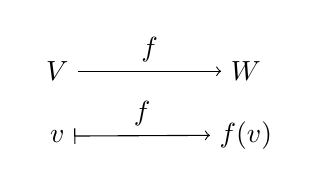
\begin{tikzpicture}
  \matrix (m) [matrix of math nodes, row sep=0.8em, column sep=4.8em, minimum width=0.2em]
  {
V & W \\
v & f(v) \\
};
  \path[->]
  (m-1-1) edge node [above] {$f$} (m-1-2)
  ;
  \path[|->]
  (m-2-1) edge node [auto] {$f$} (m-2-2)
;
\end{tikzpicture}

Consider

\[
\begin{aligned}
  & G \times \text{Hom}_k(V,W) \to \text{Hom}_k(V,W) \\ 
  & (g\cdot f) \mapsto (\sigma_g f) \circ \rho_{g^{-1}} \text{ i.e. } (g\cdot f)(v) = \sigma_gf(\rho_{g^{-1}}v) \quad \, (f\in \text{Hom}_k(V,W))
\end{aligned}
\]
Let $g,h \in G$, 
\[
(gh \cdot f)(v) = g\cdot \sigma_h f(\rho_{h^{-1}}v) = \sigma_g\sigma_h f\rho_{h^{-1}} \rho_{g^{-1}}(v) = (\sigma_{gh} f \rho_{(gh)^{-1}} )(v)
\]

Thus,  $\begin{aligned} & \quad \\
  & G \times \text{Hom}_k(V,W) \to \text{Hom}_k(V,W) \\ 
  & (g\cdot f) \mapsto (\sigma_g f)\circ \rho_{g^{-1}} \end{aligned}$ is thus another $G$-representation of $G$.  

For $k$-representation $\rho$, if the only $G$-subspaces of $V$ are $\lbrace 0 \rbrace$, $V$, $\rho$ \textbf{irreducible} or \textbf{simple}.  
\[
\begin{aligned}
  & \rho_g(\lbrace 0 \rbrace) = \lbrace 0 \rbrace \\ 
  &  \rho_g(V) = V
\end{aligned}
\]


given subrepresentation $W \subseteq V$, $V/W$ admits linear action of $G$, $\overline{\rho}_W : G \to GL_k(V/W)$ quotient representation 
\[
\overline{\rho}_W(g)(v+W) = \rho(g)(v) + W
\]
if $v'-v \in W$
\[
\rho(g)(v') + W = \rho(g)(v+(v'-v))+W = (\rho(g)(v) + \rho(g)(v'-v) ) + W = \rho(g)(v) + W
\]
\begin{proposition}[2.7 Baker (2011)\cite{ABaker2011}] \label{Prop:Baker2.7}
if $f:V \to W$ $G$-homomorphism, then
\begin{enumerate}
  \item[(a)] $\text{ker}{f}$ is $G$-subspace of $V$ 
\item[(b)] $\text{im}{f}$ is $G$-subspace of $W$
\end{enumerate}
\end{proposition}

\begin{proof}
Recall 
\begin{tikzpicture}
  \matrix (m) [matrix of math nodes, row sep=3.8em, column sep=4.8em, minimum width=2.2em]
  {
V & W \\
V & W \\
};
  \path[->]
  (m-1-1) edge node [above] {$f$} (m-1-2)
          edge node [left] {$\rho_g$} (m-2-1)
  (m-1-2) edge node [auto]  {$\sigma_g$} (m-2-2)
  (m-2-1) edge node [auto]  {$f$} (m-2-2)
  ;
\end{tikzpicture}

\begin{enumerate}
\item[(a)] Let $v\in \text{ker}{f}$.  Then $\forall \, g \in G$, 
\[
f(\rho_g v) = \sigma_g f(v) = 0 
\]
so $\rho_g v \in \text{ker}{f}$, $\forall \, g \in G$.  So $\text{ker}{f}$ is $G$-subspace of $V$
\item[(b)] Let $w\in \text{im}{f}$.  So $w = f(u)$ for some $u \in V$ 
\[
\sigma_g w = \sigma_g f(u) = f(\rho_gu) \in \text{im}f
\]
So $\text{im}{f}$ is $G$-subspace of $W$
\end{enumerate}
\end{proof}

\begin{theorem}[Schur's Lemma]
Let $\begin{aligned} & \quad \\
  & \rho : G \to GL_{\mathbb{C}}(V) \\
  & \sigma : G \to GL_{\mathbb{C}}(W) \end{aligned}$ be irreducible representations of $G$ over field $k= \mathbb{C}$; let $f:V \to W$ be $G$-linear map.  

\begin{enumerate}
  \item[(a)] if $f\neq 0$, $f$ isomorphism.  True $\forall \, k$ field, not just $\mathbb{C}$
  \item[(b)] if $V=W$, $\rho = \sigma$, then for some $\lambda \in \mathbb{C}$, $f$ given by $f(v) = \lambda v$ ($v\in V$) (true for algebraically closed fields)
\end{enumerate}
\end{theorem}

\begin{proof}
\begin{enumerate}
\item[(a)] By Prop. \ref{Prop:Baker2.7}, $\text{ker}f \subseteq V$, $\text{im}f \subseteq W$ are $G$-subspaces.  \\
For $\rho$, only $G$-subspaces are $0$ or $V$, so if $\text{ker}f = V$, $f=0$.  If $\text{ker}f = 0$, $f$ injective.  \\
For $\sigma$, only $G$-subspaces are $0$ or $V$, so $\text{im}f =0 $, $f=0$.  If $\text{im}f =V$, $f$ surjective.  

$\Longrightarrow f$ isomorphism.  
\item[(b)] Let $\lambda \in \mathbb{C}$ be an eigenvalue of $f$, $f(v_0) = \lambda v_0$ eigenvector, $v_0 \neq 0$.  

Let linear $f_{\lambda} : V \to V$ s.t. 
\[
f_{\lambda}(v) = f(v) - \lambda v \quad \, (v\in V)
\]
$\forall \, g \in G$
\[
\rho_g f_{\lambda}(v) = \rho_gf(v) - \rho_g \lambda v = f(\rho_g v) - \lambda \rho_g v= f_{\lambda}(\rho_g v)
\]
So $f_{\lambda}$ is $G$-linear, for 

\begin{tikzpicture}
  \matrix (m) [matrix of math nodes, row sep=3.8em, column sep=4.8em, minimum width=2.2em]
  {
V & V \\
V & V \\
};
  \path[->]
  (m-1-1) edge node [above] {$f$} (m-1-2)
          edge node [left] {$\rho_g$} (m-2-1)
  (m-1-2) edge node [auto]  {$\rho_g$} (m-2-2)
  (m-2-1) edge node [auto]  {$f$} (m-2-2)
  ;
\end{tikzpicture}

Since $f_{\lambda}(v_0) =0$, by Prop. \ref{Prop:Baker2.7}, $\text{ker}f_{\lambda} = V$, (for $\text{ker}f_{\lambda}\neq 0$ and so $\text{ker}f_{\lambda}=V$)

By rank-nullity theorem, $\text{dim}V = \text{dim}\text{ker}f_{\lambda} + \text{dim}\text{im}f_{\lambda}$.  

So $\text{im}f_{\lambda}=0$, and so $f_{\lambda}(v)=0$ ($\forall \, v \in V$) $\Longrightarrow f(v) = \lambda v$
\end{enumerate}
\end{proof}

Schur's lemma, at least the first part, implies that the left $kG$-modules associated with representations $\rho, \sigma$ are $kG$-isomorphic, i.e.

\[
\begin{gathered}
\begin{tikzpicture}
  \matrix (m) [matrix of math nodes, row sep=3.8em, column sep=4.8em, minimum width=2.2em]
  {
V & W \\
V & W \\
};
  \path[->]
  (m-1-1) edge node [above] {$f$} (m-1-2)
          edge node [left] {$\rho_g$} (m-2-1)
  (m-1-2) edge node [auto]  {$\sigma_g$} (m-2-2)
  (m-2-1) edge node [auto]  {$f$} (m-2-2)
  ;
\end{tikzpicture}  \Longleftrightarrow  V^{\rho} \overset{f}{\simeq} V^{\sigma}
\end{gathered}
\]

with $f$ being an isomorphism between $V^{\rho}$ and $V^{\sigma}$ s.t. 
\[
\begin{gathered}
  f(v+w) = f(v) + f(w) \quad \, \forall \, v,w \in (V^{\sigma},+) \\ 
  f(rv) = rf(v) \quad \, \forall \, r  = \sum_{g \in G} a_g g \in kG
\end{gathered}
\]

Kosmann-Schwarzbach's \textbf{Groups and Symmetries}\cite{YKosmann-Schwarzbach2010} is a very lucid text that's mathematically rigorous enough and practical for physicists.  It's really good and very clear.  Let's follow its development for $SU(2), SO(3), SL(2,\mathbb{C})$ and corresponding Lie algebras $\mathfrak{su}(2)$, $\mathfrak{so}(3)$, $\mathfrak{sl}(2,\mathbb{C})$.  

From Chapter 2 ``Representations of Finite Groups'' of Kosmann-Schwarzbach (2010) \cite{YKosmann-Schwarzbach2010}

\begin{definition}[2.1 Kosmann-Schwarzbach (2010)\cite{YKosmann-Schwarzbach2010}] \label{Def:2.1scalarproductG}
  On $L^2(G)$, scalar product defined by 
\[
\langle f_1 | f_2 \rangle = \frac{1}{|G|} \sum_{g\in G} \overline{f_1(g)} f_2(g)
\]
$f_1,f_2 \in \mathcal{F}(G) \equiv \mathbb{C}[G]$ vector space of functions on $G$ taking values on $\mathbb{C}$
\end{definition}

\begin{definition}[2.3 Kosmann-Schwarzbach (2010)\cite{YKosmann-Schwarzbach2010}]
  Let $(E,\rho)$ be representation of $G$ \\
  character of $\begin{aligned} & \quad \\ 
     \rho \equiv \chi_{\rho} & : G \to \mathbb{C} \\
     \chi_{\rho}(g) & = \text{tr}( \rho(g)) = \sum_{i=1}^n (\rho(g))_{ii} \end{aligned}$ 

Note: equivalent representations have same character \\
each conjugacy class of $G$, function $\chi_p$ is constant
\end{definition}

Looking at Def. \ref{Def:2.1scalarproductG}
\[
\langle \chi_{\rho_1} | \chi_{\rho_2} \rangle = \frac{1}{|G| } \sum_{g\in G} \chi_{\rho_1}(g^{-1}) \chi_{\rho_2(g)}
\]
since $\overline{\chi_{\rho_1(g)}} = \chi_{\rho_1}(g^{-1})$ by unitarity of representation with respect to scalar product $\langle \, , \, \rangle$

\begin{proposition}[2.7 Kosmann-Schwarzbach (2010)\cite{YKosmann-Schwarzbach2010}]
  Let $\begin{aligned} & \quad \\ 
    & (E_1, \rho_1) \\
    & (E_2, \rho_2) \end{aligned}$ be representations of $G$, let linear $u: E_1 \to E_2$.  

Then $\exists \, $ linear $T_u$ s.t. 

\begin{equation}\label{Eq:T_ucharacters}
\begin{aligned} & \quad \\
  & T_u : E_1 \to E_2 \\
  & T_u = \frac{1}{|G|} \sum_{g\in G} \rho_2(g)u\rho_1(g)^{-1} \end{aligned}
\end{equation}

so that $\rho_2(g) T_u = T_u\rho_1(g) \quad \, \forall \, g \in G$
\end{proposition}

\begin{proof}
  \[
  \rho_2(g) T_u = \frac{1}{|G|} \sum_{ h \in G } \rho_2(gh) u \rho_1(h^{-1}) = \frac{1}{|G|} \sum_{ k \in G} \rho_2(k) u \rho_1(k^{-1}g) = T_u \rho_1(g)
\]
\end{proof}

Thus, diagrammatically, we have that 
\[
\begin{tikzpicture}
  \matrix (m) [matrix of math nodes, row sep=3.8em, column sep=4.8em, minimum width=2.2em]
  {
E_1 & E_2 \\
};
  \path[->]
  (m-1-1) edge node [above] {$u$} (m-1-2)
  ;
\end{tikzpicture} \Longrightarrow  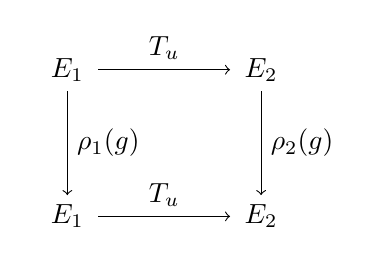
\begin{tikzpicture}
  \matrix (m) [matrix of math nodes, row sep=3.8em, column sep=4.8em, minimum width=2.2em]
  {
E_1 & E_2 \\
E_1 & E_2 \\
};
  \path[->]
  (m-1-1) edge node [above] {$T_u$} (m-1-2)
          edge node [auto] {$\rho_1(g)$} (m-2-1)
  (m-1-2) edge node [auto]  {$\rho_2(g)$} (m-2-2)
  (m-2-1) edge node [auto]  {$T_u$} (m-2-2)        
  ;
\end{tikzpicture}
\]

From Definition	1.12 of	Kosmann-Schwarzbach \cite{YKosmann-Schwarzbach2010}, ``representations $\rho_1$ and $\rho_2$ are called \textbf{equivalent} if there is a bijective intertwining operator for $\rho_1$ and $\rho_2$.''  So I will interpret this as if an intertwining operator is not bijective, then the representations $\rho_1$, $\rho_2$ are not equivalent.  

\begin{proposition}[2.8 Kosmann-Schwarzbach (2010)\cite{YKosmann-Schwarzbach2010}]
Let $\begin{aligned}
  & \quad \\
  & (E_1,\rho_1) \\
  & (E_2,\rho_2) \end{aligned}$ be irreducible representations of $G$, let linear $u:E_1 \to E_2$, define $T_u$ by $T_u = \frac{1}{ |G|} \sum_{g\in G} \rho_2(g) u \rho_1(g)^{-1}$ by Eq. \ref{Eq:T_ucharacters}.  

\begin{enumerate}
  \item[(i)] If $\rho_1$, $\rho_2$ inequivalent, then $T_u=0$
\item[(ii)] If $E_1=E_2= E$ and $\rho_1 = \rho_2 = \rho$, then
\[
T_u = \frac{\text{tr}{(u)}}{ \text{dim}E} 1_E
\]
\end{enumerate}
\end{proposition}

\begin{proof}
\begin{enumerate}
\item[(i)] if $\rho_1,\rho_2$ are inequivalent, by definition, $T_u$ is not isomorphic.  Then by Schur's lemma (first part), $T_u=0$
\item[(ii)] By Schur's lemma, $T_u(v) = \lambda v$ \, $\forall \, v \in E = E_1 = E_2$.  So $T_u = \lambda 1_E$.  $\text{tr}T_u = \lambda \text{dim}E$ or $\lambda = \frac{ \text{tr}T_u}{ \text{dim}E}$.  Thus, $T_u = \frac{\text{tr}{T_u}}{ \text{dim}E}1_E$
\end{enumerate}
\end{proof}

Let $\begin{aligned} & \quad \\
  & (e_1 \dots e_n) \text{ basis of $E$ } \\
  & (f_1 \dots f_p) \text{ basis of $F$ } \end{aligned}$ 

$\forall \, u \in \mathcal{L}(E,F)$, $\begin{aligned} & \quad \\
  & u : E \to F \\
  & u(x) = u(x^j e_j) = x^ju(e_j) = x^ju^i_{ \,\, j}f_i \\
  & u = u^i_{ \,\, j} e^j \otimes f_i \end{aligned}$ for $\begin{aligned} & \quad \\ 
  & x = x^j e_j \in E \\
  & y = y^i f_i \in F \end{aligned}$

For 
\[
\begin{aligned}
  & T : E^* \otimes F \to \mathcal{L}(E,F) \\
  & T(\xi \otimes y) = u^i_{ \,\,j}e^j \otimes f_i \text{ i.e. set $T(\xi \otimes y)$ to this $u$} \\
  & T(\xi \otimes y) = T(\xi_l e^l \otimes y^k f_k) = \xi_l y^k T(e^l \otimes f_k) = (\xi_l y^k T^{li}_{ \,\, kj} ) e^j \otimes f_i \Longrightarrow \xi_l y^k T^{li}_{ \,\, kj} = u^i_{ \,\, j}
\end{aligned}
\]

\subsubsection*{Exercises}

Exercises of Ch. 2 Representations of Finite Groups \cite{YKosmann-Schwarzbach2010}

\exercisehead{2.6}\cite{YKosmann-Schwarzbach2010} \emph{The dual representation}.  

Let $(E,\pi)$ representation of group $G$.  \\
$\forall \, g \in G$, $\xi \in E^*$, $x\in E$, set $\langle \pi^*(g)(\xi), x \rangle = \langle \xi, \pi(g^{-1})(x) \rangle$
\begin{enumerate}
\item[(a)] \emph{dual} (or \emph{contragredient}) of $\pi$, $\pi^*:G \to \text{End}(E^*)$, $\pi^*$ is a representation, since
\[
\begin{gathered}
  \langle \pi^*(gh)(\xi),x\rangle = \langle \xi, \pi((gh)^{-1})(x) \rangle = \langle \xi, \pi(h^{-1}g^{-1})(x) \rangle = \langle \xi, \pi(h^{-1}) \pi(g^{-1})(x) \rangle = \langle \xi, \pi(h^{-1}) (\pi(g^{-1})(x)) \rangle =  \\
= \langle \pi^*(h)(\xi), \pi(g^{-1})(x) \rangle = \langle \pi^*(g)\pi^*(h)(\xi), x \rangle
\end{gathered}
\]
since this is true, $\forall \, x \in E$, $\forall \, \xi \in E^*$, $\pi^*(gh) = \pi^*(g)\pi^*(h)$.  

dual $\pi^*$ of $\pi$ is a representation.  

\item[(b)]

Consider $\begin{aligned} & \quad \\
  & G \times \mathcal{L}(E,F) \to \mathcal{L}(E,F) \\
  & g\cdot u = \rho(g) \circ u \circ \pi(g^{-1}) \end{aligned}$.  

Define 
\[
\begin{aligned}
  & \sigma : G \to \text{End}(\mathcal{L}(E,F)) \\ 
  & \sigma(g):\mathcal{L}(E,F) \to \mathcal{L}(E,F) \\  
  & \sigma(g)(u) = \rho(g)\circ u \circ \pi(g^{-1})
\end{aligned}
\]

Let $(e_1 \dots e_n)$ be a basis of $E$.  Let $\xi = \xi_i e^i \in E^*$, $x = x^j e_j \in E$.  

Consider the isomorphism $T: E^*\otimes F \to \mathcal{L}(E,F)$ defined as\footnote{\emph{Mathematics stackexchage} \href{http://math.stackexchange.com/questions/428185/isomorphism-between-hom-and-tensor-product}{Isomorphism between Hom and tensor product [duplicate]} \url{http://math.stackexchange.com/questions/428185/isomorphism-between-hom-and-tensor-product} \\ \url{http://math.stackexchange.com/questions/57189/understanding-isomorphic-equivalences-of-tensor-product}}
 
\[
\begin{aligned}
  & T: E^*\otimes F \to \mathcal{L}(E,F) = \text{Hom}(E,F) \\
  & \xi \otimes y  \mapsto (x \mapsto \xi(x)y)
\end{aligned}
\]

Choose bases $\begin{aligned} & \quad \\
  & (e_1 \dots e_n) \text{ of } E \\
   & (e^1 \dots e^n) \text{ of } E^* \\  
    & (f_1 \dots f_p) \text{ of } F 
\end{aligned}$.  Then
\[
\begin{aligned}
  & T(e^j\otimes f_i)(x) = T(e^j\otimes f_i)(x^ke_k) = \delta^j_{\,\,k} x^k f_i = x^j f_i \\
  & T(e^j\otimes f_i)(e_k) = \delta^j_{\,\,k}f_i
\end{aligned}
\]

Consider 
\[
\begin{aligned} & \quad \\
  & u \in \mathcal{L}(E,F) \\
  & u: E \to F \\
  & u(x) = u(x^je_j) = x^ju(e_j) = x^j u^i_{\,\,j} f_i \\
  & u(e_j) = u^i_{\,\,j}f_i \text{ i.e. } u: e_j \to u^i_{\,\,j}f_i \end{aligned}
\]

Then $\forall u \in \mathcal{L}(E,F)$,
\[
\begin{gathered}
  T(u^i_{\,\, j} e^j \otimes f_i)(e_k) = u^i_{\,\,j}\delta^j_{\,\,k}f_i = u^i_{\,\,k}f_i = u(e_k) \Longrightarrow u = T(u^i_{\,\,j}e^j\otimes f_i)
\end{gathered}
\]
so $T$ is surjective.  

With $T(\xi\otimes y) = T(\xi'\otimes y')$, 
\[
\begin{gathered}
  T(\xi\otimes y)(x) = T(\xi' \otimes y')(x) \\
  \xi(x)y = \xi'(x)y' \Longrightarrow \xi(x)y - \xi'(x)y' = 0 
\end{gathered}
\]
which implies that $\xi\otimes y = \xi'\otimes y'$.  So $T$ is injective.  Or, one could consider that $T^{-1} : \mathcal{L}(E,F) \to E^*\otimes F$, $T^{-1} : u \mapsto u^i_{\,\,j}e^j\otimes f_i$, which is the inverse of $T$.  

\begin{remark}
\[
\begin{aligned}
  & E^* \otimes F \overset{T}{\simeq} \mathcal{L}(E,F) = \text{Hom}(E,F) \\ 
  & (\xi, y) \mapsto (x \mapsto \xi(x)y) 
\end{aligned}
\]
and so $(e^j \otimes f_i) \mapsto (x\mapsto e^j(x)f_i = x^jf_i)$

So $E^*\otimes F$ is isomorphic to $\mathcal{L}(E,F) = \text{Hom}(E,F)$
\end{remark}

For representation $\pi$, 
\[
\begin{aligned}
  & \pi:G \to \text{End}(E) \\ 
  & \pi(g):E \to E \\ 
  &  \pi(g)(x) = \pi(g)(x^j e_j) = x^j \pi(g)(e_j) = x^j \pi(g)^i_{ \,\, j} e_i = (\pi(g)^i_{\,\,j} x^j e_i
\end{aligned}
\]

Consider this matrix formulation:
\[
\begin{gathered}
  \pi^*(g)(\xi) = \pi^*(g)(\xi_i e^i) = \xi_i \pi^*(g)(e^i) = \xi_i (\pi^*(g))^i_{\,\,j}e^j \\
  \Longrightarrow \langle \pi^*(g)(\xi), x \rangle = \xi_i (\pi^*(g))^i_{ \,\, j}x^j
\end{gathered}
\]
and 
\[
\langle \xi, \pi(g^{-1})(x) \rangle = \xi_i \pi(g^{-1})^i_{ \,\, j}x^j 
\]
so that 
\[
\langle \pi^*(g)(\xi),x \rangle = \langle \xi, \pi(g^{-1})(x) \rangle \Longrightarrow \pi(g^{-1})^i_{\,\, j} = (\pi^*(g))^i_{ \,\, j}
\]
Thus, given a choice of basis for $E$, the \emph{dual} of $\pi$, $\pi^*(g)^i_{\,\,j}$, and $\pi(g^{-1})^i_{\,\,j}$ are formally equal.  

So for a choice of basis of $E$ and of $F$, 
\[
\begin{gathered}
  (\pi^*\otimes \rho)(g)(\xi,y) = (\pi^*(g)\otimes \rho(g))(\xi,y) = \pi^*(g)\xi \otimes \rho(g)y = \xi_l \pi(g^{-1})^l_{\,\,j} e^j \otimes \rho(g)^i_{\,\,k}y^k f_i = \rho(g)^i_{\,\,k}y^k \xi_l \pi(g^{-1})^l_{\,\,j} e^j \otimes f_i
\end{gathered}
\]
Applying $T$,
\[
T(\pi^*\otimes \rho)(g)(\xi,\rho) = \rho(g)^i_{\,\,k} y^k \xi_l \pi(g^{-1})^l_{\,\,j} = \rho(g)T(\xi,y) \pi(g^{-1})
\]

Thus 
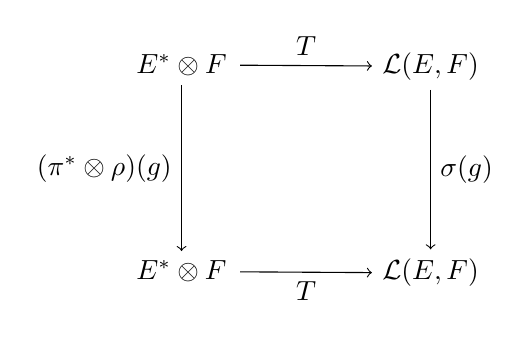
\begin{tikzpicture}
  \matrix (m) [matrix of math nodes, row sep=5.8em, column sep=4.8em, minimum width=4.2em]
  {
    E^*\otimes F & \mathcal{L}(E,F) \\ 
    E^*\otimes F & \mathcal{L}(E,F) \\ 
};
  \path[->]
  (m-1-1) edge node [above] {$T$} (m-1-2)
          edge node [left] {$(\pi^*\otimes \rho)(g)$} (m-2-1)
  (m-1-2) edge node [auto]  {$\sigma(g)$} (m-2-2)
  (m-2-1) edge node [below] {$T$} (m-2-2)
  ;
\end{tikzpicture} \quad \quad \quad \, 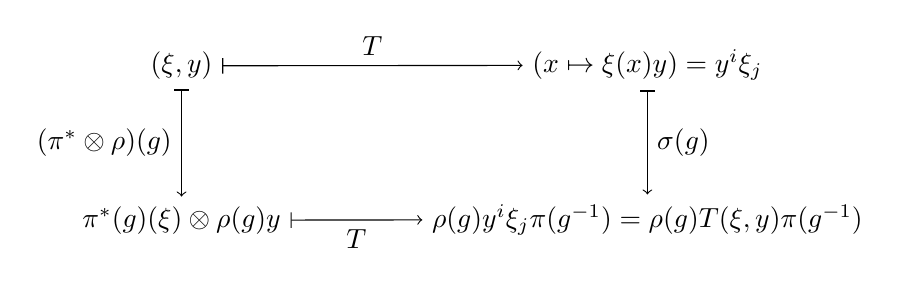
\begin{tikzpicture}
  \matrix (m) [matrix of math nodes, row sep=3.8em, column sep=4.8em, minimum width=2.2em]
  {
(\xi,y) & (x\mapsto \xi(x) y) = y^i \xi_j \\
\pi^*(g)(\xi) \otimes \rho(g)y & \rho(g) y^i \xi_j \pi(g^{-1}) = \rho(g) T(\xi,y) \pi(g^{-1}) \\
};
  \path[|->]
  (m-1-1) edge node [above] {$T$} (m-1-2)
          edge node [left] {$(\pi^*\otimes \rho)(g)$} (m-2-1)
  (m-1-2) edge node [auto]  {$\sigma(g)$} (m-2-2)
  (m-2-1) edge node [below] {$T$} (m-2-2)
  ;
\end{tikzpicture}
Thus, representation $\sigma(g)$ is equivalent to representation $(\pi^*\otimes \rho)$, a tensor product of representations.  

\end{enumerate}

\exercisehead{2.15} \emph{Representation of $GL(2, \mathbb{C})$ on the polynomials of degree 2}

Let group $G$, let representation $\rho$ of $G$ on $V= \mathbb{C}^n$, i.e. $\rho : G \to \text{End}(V)$ \\
Let $P^{(k)}(V)$ vector space of complex polynomials on $V$ that are homogeneous of degree $k$. 

For $f\in P^{(k)}(V)$, the general form is 
\[
f = \sum_{ \substack{ i_1 + i_2 + \dots + i_n = k \\ 0 \leq i_j \leq k } } a_{i_1 i_2 \dots i_d} x_1^{i_1} x_2^{i_2} \dots x_n^{i_n}
\]

Given 
\[
\binom{n+k}{k} = \binom{k-1}{k-1} + \binom{k}{k-1} + \dots + \binom{n+k-1}{k-1} = \sum_{i=0}^n \binom{k-1+i}{k-1}
\]
$\binom{k+n-1}{n-1}$ is number of monomials of degree $k$.  

So $\text{dim}P^{(k)}(V) = \binom{k+n-1}{n-1}$.   This is a very lucid and elementary exposition on the basics of polynomials which I found was useful for the basic facts I forgot\footnote{Polynomials. Math 4800/6080 Project Course \url{http://www.math.utah.edu/~bertram/4800/PolyIntroduction.pdf}}.

So we have the graded algebra
\[
P(V) = \bigoplus_{k=0}^{\infty} P^{(k)}(V)
\]

\[
\begin{aligned}
  & \rho^{(k)}: G \to \text{End}(P^{(k)}(V)) \\ 
  & \rho^{(k)}(g): P^{(k)}(V) \to P^{(k)}(V) \\ 
  & \rho^{(k)}(g)(f) = f\circ \rho(g^{-1})
\end{aligned}
\]
This is a representation of $G$ since 
\begin{enumerate}
\item[(a)] 
\[
\begin{gathered}
  \begin{aligned}
    & \rho^{(k)}(gh)(f) = f\circ \rho((gh)^{-1}) = f\circ \rho(h^{-1}g^{-1}) = f\circ \rho(h^{-1}\rho(g^{-1}) \\ 
    & \rho^{(k)}(g) \rho^{(k)}(h)(f) = \rho^{(k)}(g) (f\circ \rho(h^{-1})) = f\circ \rho(h^{-1})\circ \rho(g^{-1})
\end{aligned} \Longrightarrow \rho^{(k)}(gh) = \rho^{(k)}(g) \rho^{(k)}(h)
\end{gathered}
\]


\item[(b)]
Choose basis $(e_1 \dots e_n)$ of $V$, $x = x^j e_j \in V$, $\rho : G \to \text{End}(V)$, and so $\rho(g)(x) = \rho(g)(x^je_j) = x^j\rho(g)(e_j)= x^j(\rho(g))^i_{ \,\, j} e_i$.  \\
With $\xi(e_i) = \xi_i \Longrightarrow \langle \xi, \rho(g^{-1})x\rangle = \xi_i x^j (\rho(g^{-1}))^i_{ \,\, j}$

$\forall \, \xi \in V^*$, $\xi = \xi_i e^i$, 
\[
\begin{gathered}
  \rho^*(g)(\xi) = \rho^*(g)(\xi_i e^i) = \xi_i \rho^*(g)^i_{\,\,j} e^j \\ 
\Longrightarrow   \langle \rho^*(g)(\xi), x \rangle = \xi_i x^j (\rho^*(g))^i_{ \,\,j} \Longrightarrow (\rho^*(g))^i_{\,\,j} = (\rho(g^{-1}))^i_{ \,\, j} 
\end{gathered}
\]

So $\forall \, f \in P^{(1)}(V)$, $x\in V$, $\rho(g^{-1})x = x^j(\rho(g^{-1}))^i_{\,\,j} e_i$.  So $f\circ \rho(g^{-1})(x) = \sum_{i=1}^n a_i(\rho(g^{-1}))^i_{\,\,j} x^j = \sum_{i=1}^n a_i(\rho^*(g))^i_{\,\,j} x^j$ \\
$\Longrightarrow \rho^{(1)}(g)(f) = f\circ \rho^*(g)$
\item[(c)] Suppose $G= GL(2,\mathbb{C})$, $V=\mathbb{C}^2$, $\rho$ fundamental representation $g= \left( \begin{matrix} a & b \\
  c & d \end{matrix} \right)$, $g^{-1} = \frac{1}{\text{det}g} \left( \begin{matrix} d & -b \\
  -c & a \end{matrix} \right)$ for $\text{det}g = ad-bc$.  

Let $k=2$, $\text{dim}P^{(2)}(\mathbb{C}^2) = \binom{2+2-1}{2-1} = \binom{3}{1} = 3$

$\forall \, f \in P^{(2)}(\mathbb{C}^2)$, $f(x,y) = Ax^2 + 2Bxy + Cy^2$ \\
Let 
\[
\begin{gathered}
  P^{(2)}(\mathbb{C}^2) \to \mathbb{C}^3 \\ 
  f(x,y) = Ax^2 + 2Bxy + Cy^2 \mapsto \left( \begin{matrix} A \\ B \\ C \end{matrix} \right) \in \mathbb{C}^3
\end{gathered}
\]
Call this transformation $T$, $T: P^{(2)}(\mathbb{C}^2) \to \mathbb{C}^3$.  

$\forall \, \left( \begin{matrix} A \\ B \\ C \end{matrix} \right) \in \mathbb{C}^3$, $f(x,y) = Ax^2 + 2Bxy + Cy^2$ and $Tf(x,y) = \left( \begin{matrix} A \\ B \\ C \end{matrix} \right)$.  $T$ surjective.  

Suppose $Tf(x,y) = Tf'(x,y)$, 
\[
\begin{gathered}
  \Longrightarrow Ax^2 + 2Bxy + Cy^2 = A'x^2 + 2B'xy + C'y^2 \\ 
  \Longrightarrow (A-A')x^2 + 2(B-B')xy + (C-C')y^2 = 0
\end{gathered}
\]
Then since the monomials form a basis, and its basis elements are independent (by definition), then $A=A'$, $B=B'$, $C=C'$.  $T$ injective.  So $T$ is bijective, an isomorphism.  

(This is all in \verb|groups.sage|)
\begin{lstlisting}
sage: P2CC.<x,y> = PolynomialRing(CC,2) # this declares a PolynomialRing of field of complex numbers, 
# of order 2 (i.e. only 2 variables for a polynomial, such as x, y)
sage: A = var('A')
sage: assume(A,''complex'')
sage: B = var('B')
sage: assume(B,''complex'')
sage: C = var('C')
sage: assume(C,''complex'')
sage: f(x,y) = A*x**2 +2*B*x*y + C*y**2

sage: a = var('a')
sage: assume(a,''complex'')
sage: b = var('b')
sage: assume(b,''complex'')
sage: c = var('c')
sage: assume(c,''complex'')
sage: d = var('d')
sage: assume(d,''complex'')
sage: g = Matrix([[a,b],[c,d]] )
sage: X = Matrix([[x],[y]])
sage: f( (g.inverse()*X)[0,0], (g.inverse()*X)[1,0] ).expand()
sage: f( (g.inverse()*X)[0,0], (g.inverse()*X)[1,0] ).expand().coefficient(x^2).full_simplify()
(C*c^2 - 2*B*c*d + A*d^2)/(b^2*c^2 - 2*a*b*c*d + a^2*d^2)
sage: f( (g.inverse()*X)[0,0], (g.inverse()*X)[1,0] ).expand().coefficient(x*y).full_simplify()
-2*(C*a*c + A*b*d - (b*c + a*d)*B)/(b^2*c^2 - 2*a*b*c*d + a^2*d^2)
sage: f( (g.inverse()*X)[0,0], (g.inverse()*X)[1,0] ).expand().coefficient(y^2).full_simplify()
(C*a^2 - 2*B*a*b + A*b^2)/(b^2*c^2 - 2*a*b*c*d + a^2*d^2)
\end{lstlisting}

So 
\[
\begin{gathered}
  \rho^{(2)}(g)(f)(x,y) = f\circ \rho(g^{-1})(x,y) = \\
  = \frac{ Cc^2 - 2Bcd + Ad^2}{(ad-bc)^2}x^2 + - 2 \frac{ (Cac + Abd - (bc+ad) B)}{(ad-bc)^2} xy + \frac{ Ca^2 - 2Bab + Ab^2 }{(ad-bc)^2 } y^2
\end{gathered}
\]

So define $\widetilde{ \rho}: G \to \text{End}(\mathbb{C}^3)$. $\widetilde{\rho}$ is a representation, for 
\[
\begin{gathered}
  \forall v = \left( \begin{matrix} A \\ B \\ C \end{matrix} \right) \in \mathbb{C}^3, \quad \, \widetilde{\rho}(gh)(v) = T \circ f \circ \rho((gh)^{-1}) = T\circ f \circ \rho(h^{-1}g^{-1}) = T\circ f \circ \rho(h^{-1}) \rho(g^{-1}) \\ 
\text{ Now } \widetilde{\rho}(h)(v) = T\circ f \circ \rho(h^{-1}) \\
\Longrightarrow \widetilde{\rho}(g) \widetilde{\rho}(h)(v) = T \circ (f\circ \rho(h^{-1}))\circ \rho(g^{-1}) = T\circ f \circ \rho(h^{-1}) \rho(g^{-1}) \text{ and so }\\
\widetilde{\rho}(gh) = \widetilde{\rho}(g) \widetilde{\rho}(h)
\end{gathered}
\]

And so 
\[
\widetilde{\rho}^*(g)(v) = Tf\rho(g^{-1})
\]
and consider this commutation diagram, that (helped me at least and) clarifies the relationships:

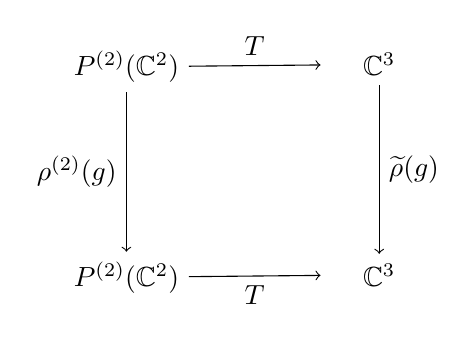
\begin{tikzpicture}
  \matrix (m) [matrix of math nodes, row sep=5.8em, column sep=4.8em, minimum width=4.2em]
  {
    P^{(2)}(\mathbb{C}^2) & \mathbb{C}^3 \\ 
    P^{(2)}(\mathbb{C}^2) & \mathbb{C}^3 \\ 
};
  \path[->]
  (m-1-1) edge node [above] {$T$} (m-1-2)
          edge node [left] {$\rho^{(2)}(g)$} (m-2-1)
  (m-1-2) edge node [auto]  {$\widetilde{\rho}(g)$} (m-2-2)
  (m-2-1) edge node [below] {$T$} (m-2-2)
  ;
\end{tikzpicture} \quad \quad \quad \, 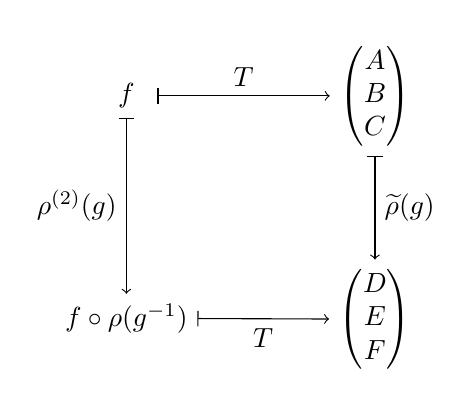
\begin{tikzpicture}
  \matrix (m) [matrix of math nodes, row sep=3.8em, column sep=4.8em, minimum width=2.2em]
  {
    f & \left( \begin{matrix} A \\ B \\ C \end{matrix} \right) \\ 
    f\circ \rho(g^{-1}) & \left( \begin{matrix} D \\ E \\ F \end{matrix} \right) \\ 
};
  \path[|->]
  (m-1-1) edge node [above] {$T$} (m-1-2)
          edge node [left] {$\rho^{(2)}(g)$} (m-2-1)
  (m-1-2) edge node [auto]  {$\widetilde{\rho}(g)$} (m-2-2)
  (m-2-1) edge node [below] {$T$} (m-2-2)
  ;
\end{tikzpicture}

with
\[
\left( \begin{matrix} D \\ E \\ F \end{matrix} \right) = \left( \begin{matrix} \frac{ Cc^2 - 2Bcd + Ad^2}{(ad-bc)^2} \\ 
- 2 \frac{ (Cac + Abd - (bc+ad) B)}{(ad-bc)^2} \\
 \frac{ Ca^2 - 2Bab + Ab^2 }{(ad-bc)^2 } \end{matrix} \right)
\]

Now define the dual $\widetilde{\rho}^*$ as such:
\[
\begin{gathered}
\begin{aligned}
  & \widetilde{\rho}^*(g): (\mathbb{C}^3)^* \to (\mathbb{C}^3)^* \\ 
  &  \widetilde{\rho}^*(g) = \widetilde{\rho}(g^{-1}) 
\end{aligned}  \\
\begin{gathered}
  \forall \, \xi \in (\mathbb{C}^3)^* \\ 
  \widetilde{\rho}^*(g)\xi = \xi_i (\widetilde{\rho}^*(g))^i_{ \,\, j} e^j = \xi_i (\widetilde{\rho}(g^{-1}))^i_{ \,\, j} e^j
\end{gathered}
\end{gathered}
\]

So for $v = \left( \begin{matrix} A \\ B \\ C \end{matrix} \right) \in \mathbb{C}^3$, $f = T^{-1}v = Ax^2 + 2Bxy + Cy^2 \in P^2(\mathbb{C}^2)$, 
\[
\widetilde{\rho}(g^{-1})(v) = T \circ ( f \rho(g) ) = \left[ \begin{matrix} Aa^2 + 2Bac + Cc^2 \\
    Aab + Bbc + Bad + Ccd \\
    Ab^2 + 2Bbd + Cd^2 \end{matrix} \right]
\]
which was found using Sage Math:
\begin{lstlisting}
sage: f((g*X)[0,0],(g*X)[1,0])
(a*x + b*y)^2*A + 2*(a*x + b*y)*(c*x + d*y)*B + (c*x + d*y)^2*C
sage: f((g*X)[0,0],(g*X)[1,0]).expand()
A*a^2*x^2 + 2*B*a*c*x^2 + C*c^2*x^2 + 2*A*a*b*x*y + 2*B*b*c*x*y + 2*B*a*d*x*y + 2*C*c*d*x*y + A*b^2*y^2 + 2*B*b*d*y^2 + C*d^2*y^2
sage: f((g*X)[0,0],(g*X)[1,0]).expand().coefficient(x^2)
A*a^2 + 2*B*a*c + C*c^2
sage: f((g*X)[0,0],(g*X)[1,0]).expand().coefficient(x*y)
2*A*a*b + 2*B*b*c + 2*B*a*d + 2*C*c*d
sage: f((g*X)[0,0],(g*X)[1,0]).expand().coefficient(y^2)
A*b^2 + 2*B*b*d + C*d^2
\end{lstlisting}
or 
\begin{lstlisting}
sage: T( f((g*X)[0,0],(g*X)[1,0]).expand() )
[A*a^2 + 2*B*a*c + C*c^2,
 2*A*a*b + 2*B*b*c + 2*B*a*d + 2*C*c*d,
 A*b^2 + 2*B*b*d + C*d^2]
\end{lstlisting}

So then 
\[
\widetilde{\rho}(g^{-1}) = \left[ \begin{matrix} a^2 & 2ac & c^2 \\ 2ab & 2(ad+bc) & 2cd \\ b^2 & 2bd & d^2 \end{matrix} \right]
\]
So then 
\[
\widetilde{\rho}^*(g) = \left[ \begin{matrix} a^2 & 2ac & c^2 \\ 2ab & 2(ad+bc) & 2cd \\ b^2 & 2bd & d^2 \end{matrix} \right]
\]
and operate on row vectors $\xi \in (\mathbb{C}^3)^*$ with $\widetilde{\rho}^*(g)$ from the row vector's right.  
\end{enumerate}

More: Let $G = SU(2)$.  Then $U = e^{i\phi} \left[ \begin{matrix} a & b \\ -\overline{b} & \overline{a} \end{matrix} \right]$

\[
\begin{gathered}
  \begin{aligned}
    & \widetilde{\rho} : SU(2) \to \text{End}(\mathbb{C}^3) \\
    & \widetilde{\rho}(U) : \mathbb{C}^3 \to \mathbb{C}^3 \\
    & \widetilde{\rho}(U)(v) = e^{-2i\varphi} \left[ \begin{matrix} A\overline{a}^2 + 2B\overline{a}\overline{b} + C \overline{b}^2 \\ 
        -A\overline{a}b + B + Ca\overline{b} \\
        Ab^2 - 2Bab + Ca^2 \end{matrix} \right]
\end{aligned} \\
  \Longrightarrow \widetilde{\rho}(U) = e^{-2i \varphi} \left[ \begin{matrix} -\overline{a}^2 & 2\overline{a}\overline{b} & \overline{b}^2 \\
      -\overline{a}b & 1 & a\overline{b} \\
      b^2 & - 2ab & a^2 \end{matrix} \right]
\end{gathered}
\]

From Chapter 4 ``Lie Groups and Lie Algebras'' of Kosmann-Schwarzbach (2010) \cite{YKosmann-Schwarzbach2010}

While Proposition 2.6 of Kosmann-Schwarzbach (2010) \cite{YKosmann-Schwarzbach2010} states that
\[
\text{det}(\exp(X)) = \exp{ (\text{tr}{X} ) }
\]
here are some other resources online that gave further discussion on the characteristic polynomial, $\text{det}(A-\lambda 1)$ and the different terms of it, called Newton identities:
\begin{itemize}
\item \url{http://scipp.ucsc.edu/~haber/ph116A/charpoly_11.pdf}
\item \url{http://math.stackexchange.com/questions/1126114/how-to-find-this-lie-algebra-proof-that-mathfraksl-is-trace-zero-matrice}
\item \url{http://mathoverflow.net/questions/131746/derivative-of-a-determinant-of-a-matrix-field}
\end{itemize}

\begin{theorem}[5.1 \cite{YKosmann-Schwarzbach2010}]\label{Thm:5.1YKos}
  Consider $\mathfrak{g} = \lbrace X = \gamma'(0) | \gamma : 1 \to G \text{ of class $C^1$ }, \, \gamma(0) = 1 \rbrace$ \\
Let Lie group $G$
\begin{enumerate}
  \item[(i)] $\mathfrak{g}$ vector subspace of $\mathfrak{gl}(n,\mathbb{R})$
  \item[(ii)] $X \in \mathfrak{g}$ iff $\forall \, t \in \mathbb{R}$, $\exp{(tX)} \in G$ 
  \item[(iii)] if $X \in \mathfrak{g}$, if $g\in G$, then $gXg^{-1} \in \mathfrak{g}$
  \item[(iv)] $\mathfrak{g}$ closed under matrix commutator, i.e. if $X,Y \in \mathfrak{g}$, $[X,Y] \in \mathfrak{g}$
\end{enumerate}
\end{theorem}

\begin{proof}
\begin{enumerate}
  \item[(i)]
\item[(ii)] If $\exp{ (tX)} \in G$, then $X \left. \frac{d}{dt} \exp{(tX)} \right|_{t=0} \in \mathfrak{g}$ (by def.)

If $X \in \mathfrak{g}$, then by def., $X = \left. \frac{d}{dt} \gamma(t) \right|_{t=0}$ with $\gamma(t) \in G$.  

Now Taylor expand; $\forall \, k \in \mathbb{Z}^+$ 

\[
\begin{gathered}
  \gamma\left( \frac{t}{k} \right) = 1 + \frac{t}{k} X + O\left( \frac{1}{k^2} \right) = \exp{ \left( \frac{t}{k} X + O\left( \frac{1}{k^2} \right) \right) } \\
  \Longrightarrow \left( \gamma \left( \frac{t}{k} \right) \right)^k = \exp{ (tX)}
\end{gathered}
\]

\[
\gamma\left( \frac{t}{k} \right) \in G \quad \, \forall \, k \in \mathbb{Z}^+
\]
$G$ closed subgroup, so $\lim_{k \to \infty} (\gamma\left( \frac{t}{k} \right) )^k = \exp{(tX) } \in G$
\item[(iii)]
\item[(iv)]
\end{enumerate}
\end{proof}

\begin{definition}
  Lie algebra $\mathfrak{g}$, tangent space to $G$ at $1$, i.e. $\mathfrak{g} := T_1 G$ is called \emph{Lie algebra} of Lie group $G$.  

\[
\mathfrak{g} := \lbrace X = \gamma'(0) | \gamma: 1 \to G \text{ of class $C^1$ }, \gamma(0) = 1 \rbrace = T_1G
\]
\end{definition}

This is based on  Proposition 5.3 of Kosmann-Schwarzbach (2010) \cite{YKosmann-Schwarzbach2010}.  

For Lie group 
\[
U(n) = \lbrace U \in GL(n,\mathbb{C}) | UU^{\dag} = 1 \rbrace
\]
If $X \in \mathfrak{u}(n)$, then $\exp{(tX)} \in U(n)$.  Then
\[
\exp{(tX)} \exp{(tX)}^{\dag} = (1+tX + O(t^2) )(1+tX^{\dag} + O(t^2) ) = 1 + t(X+X^{\dag}) +O(t^2) = 1 \forall \, t\in \mathbb{R} \Longrightarrow X+X^{\dag} = 0 
\]
i.e. $X \in \mathfrak{u}(n)$ is an anti-Hermitian complex $n\times n$ matrix.  

$\mathfrak{u}(n) = \lbrace X \in \mathfrak{gl}(n,\mathbb{C}) | X + X^{\dag} =0 \rbrace$

\emph{Physicists}: $X = iA$ and so $A-A^{\dag}$.  $A \in \mathfrak{u}(n)$ is a Hermitian complex $n\times n$ matrix.  

$\mathfrak{u}(n) = \lbrace A \in \mathfrak{gl}(n,\mathbb{C}) | A - A^{\dag} =0 \rbrace$

Regardless, $\text{dim}_{\mathbb{R}}\mathfrak{u}(n) = n^2 = 2n^2 - n^2$

For Lie group 
\[
SU(n) = \lbrace  U \in GL(n,\mathbb{C}) | UU^{\dag} = 1 , \text{det}U = 1 \rbrace
\]
Then
\[
\mathfrak{su}(n) = \lbrace X \in \mathfrak{gl}(n,\mathbb{C}) | X + X^{\dag} = 1 , \, \text{tr}{X} = 0 \rbrace
\]
is the Lie algebra of traceless anti-Hermitian complex $n\times n$ matrices, and that 
\[
\text{dim}_{\mathbb{R}}\mathfrak{su}(n) = n^2 - 1 
\]

In summary, 

\[
\begin{gathered}
  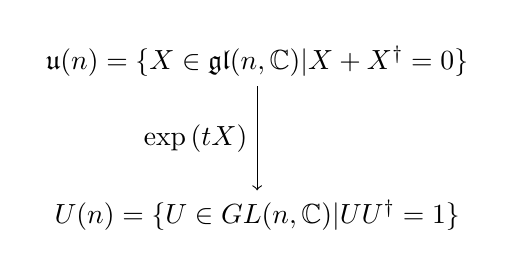
\begin{tikzpicture}
  \matrix (m) [matrix of math nodes, row sep=3.8em, column sep=4.8em, minimum width=2.2em]
  {
    \mathfrak{u}(n) = \lbrace X \in \mathfrak{gl}(n,\mathbb{C}) | X + X^{\dag} =0 \rbrace \\  
    U(n) = \lbrace U \in GL(n,\mathbb{C}) | UU^{\dag} = 1 \rbrace \\  
};
  \path[->]
  (m-1-1) edge node [left] {$\exp{(tX)}$} (m-2-1)
  ;
\end{tikzpicture} \quad \quad \, 
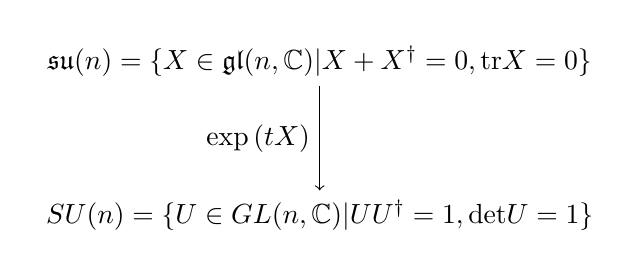
\begin{tikzpicture}
  \matrix (m) [matrix of math nodes, row sep=3.8em, column sep=4.8em, minimum width=2.2em]
  {
\mathfrak{su}(n) = \lbrace X \in \mathfrak{gl}(n,\mathbb{C}) | X + X^{\dag} =0, \text{tr}{X}=0 \rbrace \\ 
SU(n) = \lbrace U \in GL(n,\mathbb{C}) | UU^{\dag} = 1, \text{det}U=1 \rbrace \\ 
};
  \path[->]
  (m-1-1) edge node [left] {$\exp{(tX)}$} (m-2-1)
  ;
\end{tikzpicture} \\
    \text{dim}_{\mathbb{R}} \mathfrak{u}(n) = n^2   \quad \quad \quad \, \text{dim}_{\mathbb{R}}\mathfrak{su}(n) = n^2-1
\end{gathered}
\]

From Chapter 5 ``Lie Groups $SU(2)$ and $SO(3)$'' of Kosmann-Schwarzbach (2010) \cite{YKosmann-Schwarzbach2010}, 

\subsubsection{Bases of $\mathfrak{su}(2)$, Subsection 1.1 of Chapter 5of Kosmann-Schwarzbach (2010) \cite{YKosmann-Schwarzbach2010}}

Recall that 

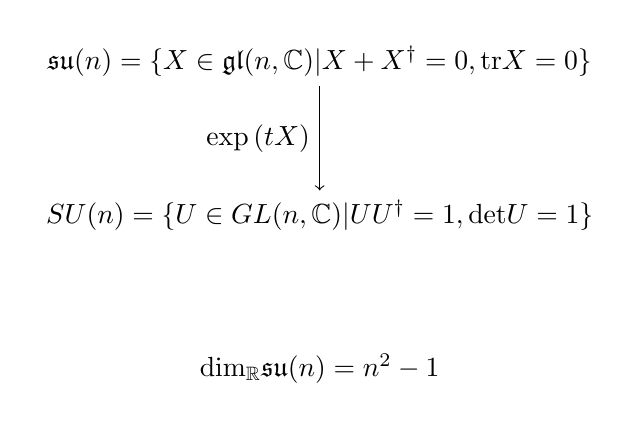
\begin{tikzpicture}
  \matrix (m) [matrix of math nodes, row sep=3.8em, column sep=4.8em, minimum width=2.2em]
  {
\mathfrak{su}(n) = \lbrace X \in \mathfrak{gl}(n,\mathbb{C}) | X + X^{\dag} =0, \text{tr}{X}=0 \rbrace \\ 
SU(n) = \lbrace U \in GL(n,\mathbb{C}) | UU^{\dag} = 1, \text{det}U=1 \rbrace \\ 
\text{dim}_{\mathbb{R}}\mathfrak{su}(n) = n^2-1 \\
};
  \path[->]
  (m-1-1) edge node [left] {$\exp{(tX)}$} (m-2-1)
  ;
\end{tikzpicture} 

and so 

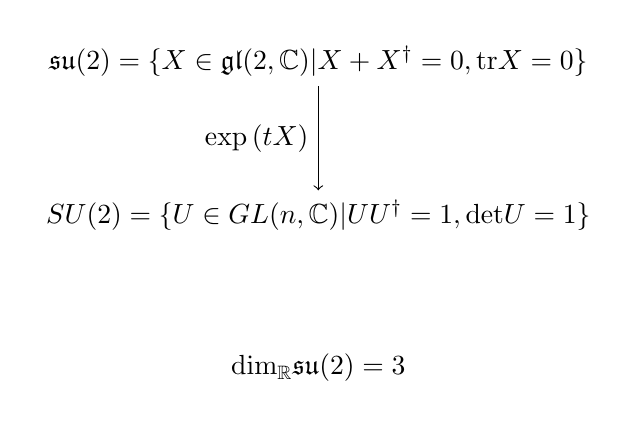
\begin{tikzpicture}
  \matrix (m) [matrix of math nodes, row sep=3.8em, column sep=4.8em, minimum width=2.2em]
  {
\mathfrak{su}(2) = \lbrace X \in \mathfrak{gl}(2,\mathbb{C}) | X + X^{\dag} =0, \text{tr}{X}=0 \rbrace \\ 
SU(2) = \lbrace U \in GL(n,\mathbb{C}) | UU^{\dag} = 1, \text{det}U=1 \rbrace \\ 
\text{dim}_{\mathbb{R}}\mathfrak{su}(2) = 3 \\
};
  \path[->]
  (m-1-1) edge node [left] {$\exp{(tX)}$} (m-2-1)
  ;
\end{tikzpicture} 

Also, recall that $\mathfrak{g} \subseteq \mathfrak{gl}(n,\mathbb{C})$ is a vector subspace (\ref{Thm:5.1YKos}) and that \\
$X \in \mathfrak{g}$ iff $\forall t \in \mathbb{R}$, $\exp{(tX)} \in G$.  \\
if $X \in \mathfrak{g}$, if $g\in G$, then $gXg^{-1} \in \mathfrak{g}$ \\
$\mathfrak{g}$ closed under $\begin{aligned} & \quad \\
  & \mathfrak{g} \times \mathfrak{g} \to \mathfrak{g} \\
 & (X,Y) \mapsto [X,Y] \end{aligned}$

and so with $\mathfrak{g}$ as a vector space, we can have a choice of bases.  

\begin{enumerate}
\item[(a)] $\begin{aligned}
  & \xi_1 = \frac{i}{2} \left( \begin{matrix} & 1 \\ 1 & \end{matrix} \right) \\ 
  & \xi_2 = \frac{1}{2} \left( \begin{matrix} & -1 \\ 1 & \end{matrix} \right) \\
  & \xi_3 = \frac{i}{2} \left( \begin{matrix} 1 &  \\  & -1 \end{matrix} \right) 
\end{aligned}$

satisfying 

\[
[\xi_k , \xi_l ] = \epsilon_{klm} \xi_m
\]
\item[(b)] \emph{Physics}

$\begin{aligned}
  & \sigma_1 = -2i \xi_1 =  \left( \begin{matrix} & 1 \\ 1 & \end{matrix} \right) \\ 
  & \sigma_2 = 2i \xi_2 =  \left( \begin{matrix} & -i \\ i & \end{matrix} \right) \\
  & \sigma_3 = -2i \xi_3 =  \left( \begin{matrix} 1 &  \\  & -1 \end{matrix} \right) 
\end{aligned}$
\end{enumerate}

satisfying 

\[
[ \sigma_k, \sigma_l ] = 2i \epsilon_{klm} \sigma_m
\]

EY : 20151001 Sage Math 6.8 doesn't run on Mac OSX El Capitan: I suspect that it's because in Mac OSX El Capitan, \verb|/usr| cannot be modified anymore, even in an Administrator account.  The TUG group for MacTeX had a clear, thorough, and useful (i.e. copy UNIX commands, paste, and run examples) explanation of what was going on:

\url{http://tug.org/mactex/elcapitan.html}

So keep in mind that my code for Sage Math is for Sage Math 6.8 that doesn't run on Mac OSX El Capitan.  I'll also use \verb|sympy| in Python as an alternative and in parallel.  

One can check in \verb|sympy| the traceless anti-Hermitian (or Hermitian) property of the bases and Pauli matrices, and the commutation relations (see \verb|groups.py|):

\begin{lstlisting}
import itertools
from itertools import product, permutations

import sympy
from sympy import I, LeviCivita
from sympy import Rational as Rat

from sympy.physics.matrices import msigma # <class 'sympy.matrices.dense.MutableDenseMatrix'>

def commute(A,B):
    """
    commute = commute(A,B)
    commute takes the commutator of A and B
    """
    return (A*B - B*A)

def xi(i):
    """
    xi = xi(i)
    xi is a function that returns the independent basis for 
    Lie algebra su(2)\equiv su(2,\mathbb{C}) of Lie group SU(2) of 
    traceless anti-Hermitian matrices, based on msigma of sympy
    cf. http://docs.sympy.org/dev/_modules/sympy/physics/matrices.html#msigma
    """
    if i not in [1,2,3]:
        raise IndexError("Invalid Pauli index")
    elif i==1:
        return I/Rat(2)*msigma(1)
    elif i==2:
        return -I/Rat(2)*msigma(2)
    elif i==3:
        return I/Rat(2)*msigma(3)

\end{lstlisting}

\begin{lstlisting}
## check anti-Hermitian property and commutation relations with xi 
# xi is indeed anti-Hermitian
xi(1) == -xi(1).adjoint() # True
xi(2) == -xi(2).adjoint() # True
xi(3) == -xi(3).adjoint() # True

# xi obeys the commutation relations

for i,j in product([1,2,3],repeat=2): print i,j

for i,j in product([1,2,3],repeat=2): print i,j, "\t Commutator: ", commute(xi(i),xi(j))

## check traceless Hermitian property and commutation relations with Pauli matrices
# Pauli matrices i.e. msigam is indeed traceless Hermitian

msigma(1) == msigma(1).adjoint() # True
msigma(2) == msigma(2).adjoint() # True
msigma(3) == msigma(3).adjoint() # True

msigma(1).trace() == 0 # True
msigma(2).trace() == 0 # True
msigma(3).trace() == 0 # True

# Pauli matrices obey commutation relation
print "For Pauli matrices, the commutation relations are :\n"
for i,j in product([1,2,3],repeat=2): print i,j, "\t Commutator: ", commute(msigma(i),msigma(j))

for i,j,k in permutations([1,2,3],3): print "Commute: ", i,j,k, msigma(i), msigma(j), \ 
": and is 2*i of ", msigma(k), commute(msigma(i),msigma(j)) == 2*I*msigma(k)*LeviCivita(i,j,k)

\end{lstlisting}

And finally the traceless property of the Pauli matrices:
\begin{lstlisting}
>>> msigma(1).trace()
0
>>> msigma(2).trace()
0
>>> msigma(3).trace()
0
\end{lstlisting} 

\subsection{Spin}

Let's follow the development by Baez and Muniain (1994) on pp. 175 of the Section II.1 ``Lie Groups'', the second (II) chapter on ``Symmetry'' \cite{JBaezJMuniain1994}.  

Let $V = \mathbb{C}^2$, $G=SU(2)$.  Then consider the graded algebra of polynomials on $V = \mathbb{C}^2 \ni (x,y)$
\[
\begin{gathered}
  P(V) = \bigoplus_{k=0}^{\infty} P^{(k)}(V) = \bigoplus_{ \substack{ j =0 \\ 2j \in \mathbb{Z}} }^{\infty} P^{(2j)}(V) = \bigoplus_{ \substack{ j=0 \\ j\in \mathbb{Z} }}^{\infty} P^{(2j)}(V) \oplus \bigoplus_{ \substack{ j=1/2 \\ 2j \text{ odd } } }^{\infty} P^{(2j)}(V) \\
  P^{(2j)}(V) \equiv \text{ vector space of complex polynomials of degree $2j$ }
\end{gathered}
\]
and recall this representation on $P^{(2j)}(V)$
\[
\begin{aligned}
  & \rho^{(2j)}:G \to \text{End}(P^{(2j)}(V)) \\ 
  & \rho^{(2j)}: P^{(2j)}(V) \to P^{(2j)}(V) \\ 
 & \rho^{(2j)}(g)(f) = f\circ \rho(g^{-1}) \text{ where $\rho$ is the fundamental representation of $G=SU(2)$ }\\
    & \rho^{(2j)}(g)(f)(v) = f\circ \rho(g^{-1})(v) \quad \, \forall \, f \in P^{(2j)}(V), \, \forall \, v \in V = \mathbb{C}^2
\end{aligned}
\]
Note, \\
$\text{dim}P^{(2j)} = \binom{2j+2-1 }{2-1} = 2j+1$

\exercisehead{21} \cite{JBaezJMuniain1994} \emph{spin-0} Consider the trivial representation $\tau$:
\[
\begin{aligned}
  & \tau : G \to \text{End}(\mathbb{C}) \\ 
  & \tau(g): \mathbb{C} \to \mathbb{C} \\ 
  & \tau(g) = 1_{\mathbb{C}}
\end{aligned} \quad \quad \,  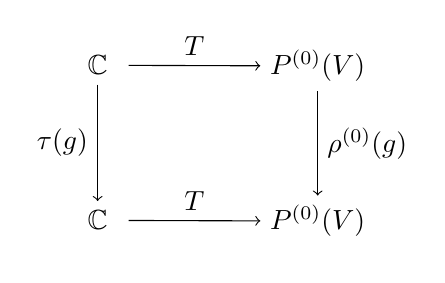
\begin{tikzpicture}
  \matrix (m) [matrix of math nodes, row sep=3.8em, column sep=4.8em, minimum width=2.2em]
  {
\mathbb{C} & P^{(0)}(V) \\ 
\mathbb{C} & P^{(0)}(V) \\ 
};
  \path[->]
  (m-1-1) edge node [above] {$T$} (m-1-2)
          edge node [left] {$\tau(g)$} (m-2-1)
  (m-1-2) edge node [auto]  {$\rho^{(0)}(g)$} (m-2-2)
  (m-2-1) edge node [auto] {$T$} (m-2-2)
  ;
\end{tikzpicture}
\]

Clearly, $P^{(0)}(V) = \mathbb{C}$, since $P^{(0)}(V)$ consists of polynomials of constants in $\mathbb{C}$.  

Consider $c_0 \in \mathbb{C}$, $f = k_0 \in P^{(0)}(V)$ \\
$\rho^{(0)}(g)(f) = f\circ \rho(g^{-1}) = k_0$ \\
$\Longrightarrow \rho^0(g)T(c_0) = T\circ \tau(g) c_0 = T(c_0)$.  Let $T = 1_{\mathbb{C}} = 1_{P^{0}(V)}$

So $\rho^{(0)}(g) = \tau(g) = 1$.  $T=1$.  So representations $\rho^{(0)}$ and trivial representation $\tau$ on $G$ are equivalent.  



\exercisehead{22} \cite{JBaezJMuniain1994} \emph{spin-$\frac{1}{2}$} For spin-$\frac{1}{2}$, $j=\frac{1}{2}$, $2j=1$.  

$\forall \, f \in P^{(1)}(V)$, $V = \mathbb{C}^2$.  So in general form, $f(x,y) = ax + by \in P^{(1)}(V)$, $\left( \begin{matrix} x \\ y \end{matrix} \right) \in V = \mathbb{C}^2$  

Recall the fundamental representation $\begin{aligned} & \quad \\
  & \rho : G \to GL(2,\mathbb{C}) \equiv GL(\mathbb{C}^2) \\
  & \rho(g) : \mathbb{C}^2 \to \mathbb{C}^2 \\
  & \rho(g) = g \end{aligned}$

So consider $T$ such that 

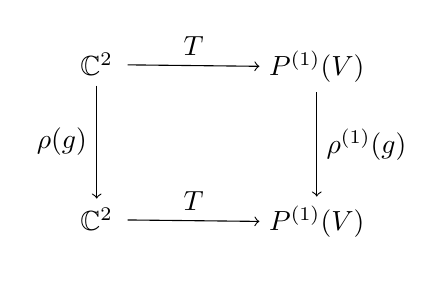
\begin{tikzpicture}
  \matrix (m) [matrix of math nodes, row sep=3.8em, column sep=4.8em, minimum width=2.2em]
  {
\mathbb{C}^2 & P^{(1)}(V) \\ 
\mathbb{C}^2 & P^{(1)}(V) \\ 
};
  \path[->]
  (m-1-1) edge node [above] {$T$} (m-1-2)
          edge node [left] {$\rho(g)$} (m-2-1)
  (m-1-2) edge node [auto]  {$\rho^{(1)}(g)$} (m-2-2)
  (m-2-1) edge node [auto] {$T$} (m-2-2)
  ;
\end{tikzpicture}

Consider $\forall \, v \in \mathbb{C}^2$, $v =\left( \begin{matrix} x \\ y \end{matrix} \right)$, then 
\[
\rho(g)v = gv = \left[ \begin{matrix} ax + by \\ cx + dy \end{matrix} \right]
\]

\begin{lstlisting}
sage: g*X
[a*x + b*y]
[c*x + d*y]
\end{lstlisting}

For notation, let $U \in G = SU(2)$ s.t. $UU^{\dag}=1$.  

Consider $(\rho^{(2j)}(U)(f))(x) = f(U^{-1}x)$, $\forall \, x \in \mathbb{C}^2$.  

Choose $f(x,y) = x$.  So for $f(x,y) = Ax+By$, $A=1,B=0$.  Choose $U = \left( \begin{matrix} a & b \\
  -\overline{b} & \overline{a} \end{matrix} \right)$ so $U^{-1} = \left( \begin{matrix} \overline{a} & -b \\
  \overline{b} & a \end{matrix} \right)$.  Then $U^{-1}x = \left( \begin{matrix} \overline{a}x - by \\
  \overline{b}x + ay \end{matrix} \right)$

So 
\[
\begin{aligned}
  & (\rho^{(1)}(U)(f) )(x) = f(U^{-1}x) = \overline{a}x - by \\ 
  & (\rho^{(1)}(U)(f))(x) = f(U^{-1}x) = \overline{b}x + ay \text{ for } f(x,y) = y 
\end{aligned}
\]
Let $f(x,y) = Ax + By$
\[
\begin{gathered}
  (\rho^{(1)}(U)(f))(x) = f(U^{-1}x) = (A\overline{a}+B\overline{b})x + (Ba - Ab)y = (\overline{a}x - by)A + (\overline{b}x + ay)B  = (A\overline{a} + B\overline{b})x + (Ba-Ab)y
\end{gathered}
\]
which was calculated with the assistance of Sage Math:
\begin{lstlisting}
sage: U_try1 = Matrix( [[a.conjugate(),-b],[b.conjugate(),a ] ] )
sage: f1( U_try1*X).coefficient(x)
A*conjugate(a) + B*conjugate(b)
sage: f1( U_try1*X).coefficient(y)
B*a - A*b
\end{lstlisting}

Treating $P^{(1)}(\mathbb{C}^2)$ as a vector space, in its matrix formulation, then $f(x,y) = Ax+By \in P^{(1)}(\mathbb{C}^2)$ is treated as $\left[ \begin{matrix} A \\ B \end{matrix} \right]$, then $(\rho^{(1)}(U)f)$ is 
\[
\Longrightarrow \left[ \begin{matrix} \overline{a} & \overline{b} \\ -b & a \end{matrix} \right]\left[ \begin{matrix} A \\ B \end{matrix} \right] = \left[ \begin{matrix} A\overline{a} + B\overline{b}  \\ -Ab + Ba \end{matrix} \right]
\]
so conclude in general that $\rho^{(1)}(U) = (U^{\dag})^T$.  

Now, as Kosmann-Schwarzbach (2010) \cite{YKosmann-Schwarzbach2010} says, on pp. 13, Chapter 2 Representations of Finite Groups, ``Two representations $(E_1,\rho_1)$ and $(E_2,\rho_2)$ are equivalent if and only if there is a basis $B_1$ of $E_1$ and a basis $B_2$ of $E_2$ such that for every $g\in G$, the matrix of $\rho_1(g)$ in the basis $B_1$ is equal to the matrix of $\rho_2(g)$ in the basis $B_2$.  In particular, if the representations $(E_1,\rho_1)$ and $(E_2,\rho_2)$ are equivalent, then $E_1$ is isomorphic to $E_2$.''  So we need a change of basis between $\rho(U) = U$ and $\rho^{(1)}(U)$.  What's the linear transformation $T$ s.t.
\[
T^{-1} \rho^{(1)}(U) T = U ?
\]  
By intuition, 
\[
T = \sigma_x \sigma_z \equiv \sigma_1 \sigma_3
\]
where $\sigma_i$'s are Pauli matrices.  

Indeed, 
\begin{lstlisting}
sage: Paulimat[3] * Paulimat[1]*U_try*Paulimat[1] * Paulimat[3]
[conjugate(a) conjugate(b)]
[          -b            a]
\end{lstlisting}

Then $\rho^{(1)}(U)\circ T = TU$, so this $T = \sigma_1 \sigma_3$ is an ``intertwining operator'' between $\rho^{(1)}(U)$ and fundamental representation $\rho(U) = U$, with $T = \left[ \begin{matrix} & - 1 \\
    1 & \end{matrix} \right]$, and $T^{-1} = \left[ \begin{matrix} & 1 \\ -1 & \end{matrix} \right]$.  

$T$ is an isomorphism between $\mathbb{C}^2$ and $P^{(1)}(\mathbb{C}^2)$.  So fundamental representation $\rho$ of $G=SU(2)$ is equivalent to $\rho^{(1)}(U)$ on $P^{(1)}(\mathbb{C}^2)$.  

\exercisehead{23}\cite{JBaezJMuniain1994} (Also from Exercise 2.6 of Kosmann-Schwarzbach (201) \cite{YKosmann-Schwarzbach2010})

Let $(E,\pi)$ representation of group $G$.  \\
$\forall \, g \in G$, $\xi \in E^*$, $x\in E$, set $\langle \pi^*(g)(\xi), x \rangle = \langle \xi, \pi(g^{-1})(x) \rangle$

 \emph{dual} (or \emph{contragredient}) of $\pi$, $\pi^*:G \to \text{End}(E^*)$, $\pi^*$ is a representation, since
\[
\begin{gathered}
  \langle \pi^*(gh)(\xi),x\rangle = \langle \xi, \pi((gh)^{-1})(x) \rangle = \langle \xi, \pi(h^{-1}g^{-1})(x) \rangle = \langle \xi, \pi(h^{-1}) \pi(g^{-1})(x) \rangle = \langle \xi, \pi(h^{-1}) (\pi(g^{-1})(x)) \rangle =  \\
= \langle \pi^*(h)(\xi), \pi(g^{-1})(x) \rangle = \langle \pi^*(g)\pi^*(h)(\xi), x \rangle
\end{gathered}
\]
since this is true, $\forall \, x \in E$, $\forall \, \xi \in E^*$, $\pi^*(gh) = \pi^*(g)\pi^*(h)$.  

dual $\pi^*$ of $\pi$ is a representation.  


\part{Bundles}

\cite{CTaubes2011}


\section{Vector bundles}

Ballmann has a lucid and straightforward and useful exposition on vector bundles and connections \cite{WBallmann1999} \footnote{Werner Ballmann. ``Vector bundles and connections'', \url{http://people.mpim-bonn.mpg.de/hwbllmnn/archiv/conncurv1999.pdf}}.  

  $\mathbb{K} \in \lbrace \mathbb{R},\mathbb{C} \rbrace$
\begin{definition}
$\mathbb{K}$-vector bundle over $M$ of rank $k$ is bundle $\pi:E \to M$, fibers $E_p := \pi^{-1}(p)$ are $\mathbb{K}$-vector spaces, s.t. \\
$\forall \, p \in M$, $\exists \, $ open $U \subseteq M$, $U \ni p$, $\exists \, $ diffeomorphism (called local trivialization) $\Phi: \left. E \right|_{\pi^{-1}(U) } \to U\times \mathbb{K}^k$ s.t. \\
\phantom{ \quad \, } $\pi \circ \Phi^{-1} = \pi_1$ \quad \, $\pi_1 : U \times \mathbb{R}^k \to U$ is canonical projection \\

\phantom{ \quad \, } $\forall \, q \in U$, $\begin{aligned} & \quad \\
  & \Phi_q^{-1}: \mathbb{K}^k \to E_q \\
  & \Phi_q^{-1}(v) := \Phi^{-1}(q,v) \end{aligned}$ is a $\mathbb{K}$-linear isomorphism.
\end{definition}








\begin{definition}\label{Prop:frametrivializequiv}
  \textbf{frame} of $E$ over $U$ is $k$-triple $(s_1 \dots s_k)$, $s_i \in \Gamma(\left. E \right|_{\pi^{-1}(U)} )$, $\sigma_i$ smooth section of $E$ over $U$ s.t. 
\[
\sigma_1(p) \dots \sigma_k(p)
\]
basis of $E_p$ \, $\forall \, p \in U$
\end{definition}

By Prop. \ref{Prop:frametrivializequiv}, frames and local trivializations are ``equivalent''.  




\begin{proposition}





conversely, if $ \Phi : \left. E \right|_{\pi^{-1}(U)} \to U \times \mathbb{K}^k$ trivialization of $\left. E \right|_{\pi^{-1}(U)}$ and $e_1 \dots e_k$ standard basis of $\mathbb{K}^k$, then $k$-tuple $\sigma_i = \Phi^{-1}(\cdot, e_i)$, $1 \leq i \leq k$ is a frame of $E$ over $U$. 
\end{proposition}




\begin{definition}
Let $\Phi^{-1} = (s_1,\dots, s^k)$ local trivialization/frame. \\
Consider arbitrary $s \in \Gamma( \left. E \right|_{\pi^{-1}(U) })$  \\
Then $\exists \, \sigma = \sigma_{\Phi^{-1} }: U \to \mathbb{K}^k$ s.t.
\[
s(p) = \Phi^{-1}(p,\sigma(p)) \quad \, \forall \, p \in U \text{ i.e. } s = \sigma^i s_i \, , \,  \sigma = (\sigma^1 \dots \sigma^k)
\] 
$\sigma$ \emph{principal part of $s$ with respect to $\Phi$}.
\end{definition}

Let $\Psi^{-1} = (t_1 \dots t_k)$ another local trivialization of $E$ over open $V \subseteq M$.  \\
\phantom{Let } $\forall \, p \in U \bigcap V$, isomorphisms $\begin{aligned} & \quad \\
  & \Phi_p^{-1} : \mathbb{K}^k \to E_k \\
  & \Psi_p^{-1} : \mathbb{K}^k \to E_k  \end{aligned}$ , \quad \, $\begin{aligned} & \quad \\
  & \Phi^{-1} = (s_1 \dots s_k) \\
  & \Psi^{-1} = (t_1 \dots t_k) \end{aligned}$, then 

\[
s_j = g^i_{ \,\, j} t_i 
\]
with smooth $g^i_{ \,\, j} : U \bigcap V \to \mathbb{K}$, $\forall \, p \in U \bigcap V$, $g^i_{ \,\, j}(p) = a^i_{ \, \, j}(p) \in \text{Mat}(k,k)$, ($k\times k$ matrix).  \\
\phantom{ with } $g^i_{ \,\, j}$ invertible so smooth $g:U\bigcap V \to Gl(k,\mathbb{K})$.

Let $s\in \Gamma(E)$ over $U\bigcap V$, $\sigma_{\Phi}$, $\sigma_{\Psi}$ principal part of $s$ with respect to $\Phi$,$\Psi$.  Then
\[
\sigma^i_{\Psi} = g^i_{ \,\, j} \sigma^j_{\Phi} \text{ i.e. } \sigma_{\Psi} = g\cdot \sigma_{\Phi}
\]

Indeed, $\forall \, s \in \Gamma(E)$,
\[
s = \sigma^j_{\Phi} s_j = \sigma^j_{\Phi} g^i_{ \,\, j} t_i = g^i_{ \,\, j} \sigma^j_{ \Phi } t_i = \sigma^i_{\Psi } t_i
\]





\[
\begin{gathered}
  \nabla_X s = (X(\sigma^i_{\Phi})+\sigma^j_{\Phi}(\omega_{\Phi})^i_{ \,\, j}(X) ) s_i = (X(\sigma^i_{\Psi}) + \sigma^j_{\Psi} (\omega_{\Psi})^i_{ \, \, j}(X) )t_i = (X(g^i_{ \,\, k} \sigma^k_{\Psi} ) + g^j_{ \,\,k} \sigma_{\Phi}^k (\omega_{\Psi})^i_{ \,\, j}(X))t_i = \\
  = X(\sigma^k_{\Phi})s_k + t_i X(g^i_{ \,\, k} ) \sigma^k_{\Phi} + t_i (\omega_{\Psi})^i_{ \,\, j}(X) g^j_{ \,\, k} \sigma^k_{\Phi} 
\end{gathered}
\]
$X(\sigma^j_{\Phi})s_i$ cancels from both sides and so
\[
\begin{gathered}
  \Longrightarrow s_i \sigma^j_{\Phi} (\omega_{\Phi})^i_{ \,\, j}(X) = s_i (\omega_{\Phi})^i_{ \,\, j}(X) (g^{-1})^j_{ \,\, k} (\sigma_{\Psi})^k = t_l g^l_{\,\, i} (\omega_{\Phi})^i_{ \,\, j}(X) (g^{-1})^j_{\,\,k} \sigma^k_{\Psi} = \\
  = t_l X(g^l_{ \,\, k})(g^{-1})^k_{ \,\, i} \sigma^i_{\Psi} + t_l (\omega_{\Psi})^l_{ \,\, j}(X) \sigma^j_{\Psi}  \\
  \Longrightarrow \omega_{\Psi}(X) = g\omega_{\Phi}(X)g^{-1} - X(g)(g^{-1})
\end{gathered}
\]

In summary, 
\begin{quote}
for connection $\begin{aligned} & \quad \\
  & \nabla : \mathfrak{X}(M) \times \Gamma(E) \to \Gamma(E) \\
  & \nabla(X,s) = \nabla_Xs = (\nabla s)(X) \in \Gamma(E) \end{aligned}$

For frames $\begin{aligned} & \quad \\
  & \Phi^{-1} = (s_1 \dots s_k) \text{ of $E$ over open $U$ } \\
  & \Psi^{-1} = (t_1 \dots t_k) \text{ of $E$ over open $V$ } 
\end{aligned}$, \, $U\cap V \neq \emptyset$, $\exists \, $ smooth $g = (g^i_{ \,\, j} ):U \cap V \to \text{Gl}(k;\mathbb{K})$ s.t. 

\[
s_j = t_i g^i_{ \,\, j} \text{ or } \Phi^{-1} = \Psi^{-1}g 
\]
Then $\forall \, s \in \Gamma(E_{\pi^{-1}(U\cap V) })$, $s = \sigma^j_{\Phi}s_j = \sigma^j_{\Psi} t_j$, so 
\[
\sigma^i_{\Psi} = g^i_{  \, \, j} \sigma^j_{\Phi} \text{ or } \sigma_{\Psi} = g\sigma_{\Phi}
\]
then
\[
\nabla_X s = s_i(X(\sigma^i) + \omega^i_{ \,\, j}(X)\sigma^j) 
\]
so that 
\begin{equation}
\boxed{ \omega_{\Psi}(X) = g\omega_{\Phi}(X)g^{-1} - X(g)(g^{-1}) \text{ or } (\omega_{\Psi})^i_{\, \, j}(X) = g^i_{ \,\, k} (\omega_{\Phi})^k_{ \,\, l }(X) (g^{-1})^l_{ \,\, j} - X(g^i_{ \,\, k})(g^{-1})^k_{ \,\, j} }
\end{equation}
\end{quote}




define covariant derivative $d\mathbf{v} = (x,\left. d\mathbf{v}\right|_x)$

$\forall \, \sigma \in \Gamma(E)$, section $\sigma$ of $E$. define
\[
\nabla \sigma = \sum_{U \in \mathcal{U}} \chi_U \varphi_U^*(d(\varphi_U \circ \left. \sigma \right|_U ) )
\]

\[
\begin{gathered}
  \nabla (f\sigma) = \sum_{U \in \mathcal{U}} \chi_U \varphi_U^*(d(\varphi_U \circ f \left. \sigma \right|_U ) )  = \sum_{U \in \mathcal{U}} \chi_U \varphi_U^*((d\varphi_U) (d (f \left. \sigma \right|_U ) ) ) = \sum_{U \in \mathcal{U}} \chi_U \varphi_U^*((d\varphi_U) ( \left. \sigma \right|_U df + f \left. d\sigma \right|_U ) = \\
=  \sum_{U \in \mathcal{U}} \chi_U \varphi_U^*(d\varphi_U) \left. \sigma \right|_U \otimes df + \sum_{U \in \mathcal{U}} \chi_U \varphi_U^*(d\varphi_U)(f \left. d\sigma  \right|_U ) = \sum_{U \in \mathcal{U}} \chi_U f \varphi_U^* d ( \varphi_U \circ \left. d\sigma  \right|_U ) +  \sum_{U \in \mathcal{U}} \chi_U \varphi_U^*(d\varphi_U) \left. \sigma \right|_U \otimes df = \\
= f\nabla \sigma + \sigma \otimes df
\end{gathered}
\]

\section{Principal bundles}

Let's follow Taubes (2011) from Chapter 10 ``Principal bundles'', on \cite{CTaubes2011}.


\begin{definition}
  Let smooth manifold $M$, Lie group $G$. \\
  \emph{principal} $G$-bundle $\equiv $ smooth manifold $P$ s.t. 
\begin{itemize}
  \item smooth action of $G$ by diffeomorphisms $\equiv$ map $m: G \times P \to P$ s.t. 
    \begin{itemize}
      \item $m(1,p) =p$
      \item $m(h,m(g,p)) = m(hg,p)$
    \end{itemize}
    Notation: $(g,p) \mapsto pg^{-1}$

EY : 20151007 note that 
\[
(g,p) \mapsto pg^{-1} \xrightarrow{m(h)} pg^{-1}h^{-1} = p(hg)^{-1} = m(hg,p)
\]
\begin{tikzpicture}
  \matrix (m) [matrix of math nodes, row sep=3.8em, column sep=4.8em, minimum width=2.2em]
  {
G\times P & G \\
P & \\
};
  \path[->]
  (m-1-1) edge node [auto] {$$} (m-1-2)
          edge node [left] {$m$} (m-2-1)
  ;
\end{tikzpicture} \quad \quad \, \begin{tikzpicture}
  \matrix (m) [matrix of math nodes, row sep=3.8em, column sep=4.8em, minimum width=2.2em]
  {
(g,p) & g \\
m(p,g) = pg^{-1} & \\
};
  \path[|->]
  (m-1-1) edge node [auto] {$$} (m-1-2)
          edge node [left] {$m$} (m-2-1)
  ;
\end{tikzpicture}
  \item projection from $P$ to $M$, $\pi \equiv $ surjective $\pi : P \to M$ that's $G$-invariant, i.e. $\pi(pg^{-1}) =p$
  \item $\forall \, p \in M$, $\exists \, $ open $U \ni p$, with $G$-equivariant diffeomorphism $\varphi : \left. P \right|_{U} \to U\times G$ s.t. \\
if $\varphi(p)  = (\pi(p), h(p))$, $h(p) \in G$, then $\varphi(pg^{-1}) = (\pi(p), h(p)g^{-1})$

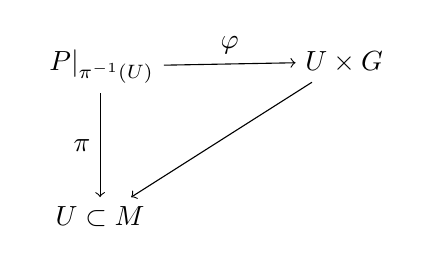
\begin{tikzpicture}
  \matrix (m) [matrix of math nodes, row sep=3.8em, column sep=4.8em, minimum width=2.2em]
  {
\left. P \right|_{\pi^{-1}(U)} & U\times G \\
U\subset M  & \\
};
  \path[->]
  (m-1-1) edge node [auto] {$\varphi$} (m-1-2)
          edge node [left] {$\pi$} (m-2-1)
  (m-1-2) edge node [auto] {$$} (m-2-1)
  ;
\end{tikzpicture} \quad \quad \, 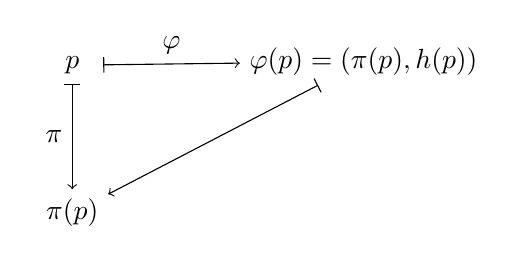
\begin{tikzpicture}
  \matrix (m) [matrix of math nodes, row sep=3.8em, column sep=4.8em, minimum width=2.2em]
  {
p & \varphi(p) = (\pi(p),h(p)) \\
\pi(p) & \\
};
  \path[|->]
  (m-1-1) edge node [auto] {$\varphi$} (m-1-2)
          edge node [left] {$\pi$} (m-2-1)
  (m-1-2) edge node [auto] {$$} (m-2-1)
  ;
\end{tikzpicture} \quad \quad \, 

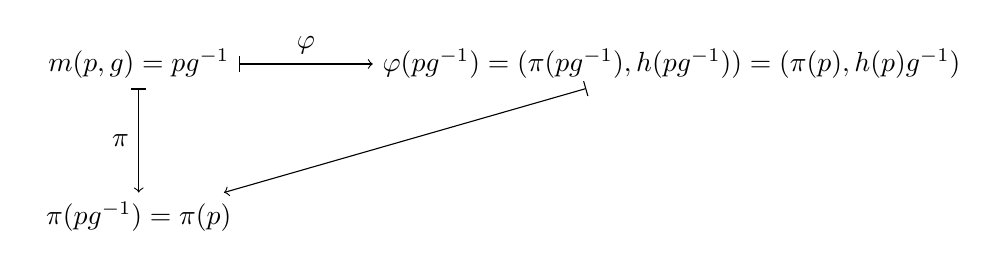
\begin{tikzpicture}
  \matrix (m) [matrix of math nodes, row sep=3.8em, column sep=4.8em, minimum width=2.2em]
  {
m(p,g) = pg^{-1} & \varphi(pg^{-1}) = (\pi(pg^{-1}), h(pg^{-1})) = (\pi(p),h(p)g^{-1}) \\
\pi(pg^{-1}) = \pi(p) & \\
};
  \path[|->]
  (m-1-1) edge node [auto] {$\varphi$} (m-1-2)
          edge node [left] {$\pi$} (m-2-1)
  (m-1-2) edge node [auto] {$$} (m-2-1)
  ;
\end{tikzpicture}
\end{itemize}
\end{definition} cf. Section 10.1 ``The definition'' of Taubes (2011) \cite{CTaubes2011}

\subsubsection{Cocycle definition (Sec. 10.2 ``A cocycle definition'') \cite{CTaubes2011} }

Let locally finite, open cover $\mathcal{U} = \lbrace U_{\alpha} \rbrace$ of $M$ (recall \emph{locally finite}: $\forall \, p \in M$, $\exists \, $ open $\mathcal{O} \ni p$ s.t. $\mathcal{O} \bigcap U_{\alpha}$ for only finite many $\alpha$'s).  

\begin{definition}
  \emph{principal bundle transition functions} $\equiv \lbrace g_{\alpha \beta} : U_{\alpha} \bigcap U_{\beta} \to G \rbrace_{U_{\alpha},U_{\beta} \in \mathcal{U}}$ i.e. collection of smooth maps from intersections of $U_{\alpha},U_{\beta} \in \mathcal{U}$ s.t. \emph{cocycle constraints} hold:
\begin{itemize}
  \item $g_{\alpha \alpha} =1$ 
  \item $g^{-1}_{\alpha \beta} = g_{\beta \alpha }$
    \item if $U_{\alpha}, U_{\beta}, U_{\gamma} \in \mathcal{U}$, $U_{\alpha} \bigcap U_{\beta} \bigcap U_{\gamma} \neq \emptyset$, $g_{\alpha \beta} g_{\beta \gamma} g_{\gamma \alpha } =1$
\end{itemize}
\end{definition}

\begin{claim}
  principle $G$-bundle $P = \coprod_{U \in \mathcal{U}} U_{\alpha} \times G / \sim$

with equivalence relation $\sim$ s.t. $\forall \, \begin{aligned} & \quad \\
  & (x,g) \in U_{\alpha} \times G \\
  & (x',g') \in U_{\beta} \times G \end{aligned}$, $(x,g) \sim (x',g')$ iff $x=x'$ and $g=g_{\alpha \beta} g'$
\end{claim}

\begin{proof}
  Let $[(x,g)] \in \coprod_{U_{\alpha} \in \mathcal{U}} U_{\alpha} \times G / \sim$

  Now for $m : G \times P \to P$, $m(h) : P \to P$ for $h\in G$, 
  \[
\begin{gathered}
  \begin{aligned}
    & [(x,g)] =(x,g) \xrightarrow{ m(h)}(x,gh^{-1}) \\ 
    & [(x,g)] = (x,g') \xrightarrow{ m(h)} (x,g'h^{-1}) = (x,g^{-1}_{\alpha \beta} gh^{-1}) = (x,g_{\beta \alpha} gh^{-1})
  \end{aligned}
\end{gathered}
\]
Now $(x,gh^{-1}) \sim (x,g_{\beta \alpha} gh^{-1})$.  So we have a well-defined smooth action of $G$ by diffeomorphisms $m: G\times P \to P$, but now on the equivalence classes of $\coprod_{U_{\alpha} \in \mathcal{U}} U_{\alpha}\times G/\sim$, i.e.
\[
[(x,g)] \xrightarrow{ m(h)} [(x,gh^{-1})]
\]  

Second, 
\[
[(x,g)] \xrightarrow{ \pi} x\in M
\]
unequivocally.  So we have a surjective projection from $P$ to $M$, $\pi$, but now a surjective projection from $\coprod_{U_{\alpha} \in \mathcal{U}} U_{\alpha}\times G/\sim$ to $M$.

% EY : 20151007 Third part, I'm not clear about and need some help.  

%Third, recall $G$-equivalent diffeomorphism $\varphi : \left. P \right|_{U} \to U \times G$ for some open $U \ni x \in M$.  Fix this $U$ to be $U$.  
%\[
%\begin{aligned}
%  & [U\times G] \xrightarrow{ \varphi } U\times G \\ 
%  & [(x,g)] \xrightarrow{ \varphi } \varphi([(x,g)]) = (\pi((x,g)), h((x,g)) ) = (x,h((x,g)) ) = (x,h(x)g^{-1})
%\end{aligned}
%\]
%I'll try to check the well-definedness:
%\[
%\begin{gathered}
%  \varphi([x,g]) = \varphi((x,g')) = \varphi((x,g_{\beta\alpha}g) ) = (x,h(x)(g_{\beta \alpha} g)^{-1}) = (x,h(x) g^{-1}g_{\beta\alpha}^{-1}) = (x,h(x)g^{-1}g_{\alpha\beta})
%\end{gathered}
%\]

Third, define a $G$-equivariant diffeomorphism as such: Let $[(x,g)] \in \coprod_{U_{\alpha} \in \mathcal{U}} U_{\alpha}\times G/\sim$.  In fact, let $[(x,g)] \in U_{\alpha}\times G/\sim$.  So $\forall \, x \in M$, $\exists \, U_{\alpha} \ni x$, $U_{\alpha} \in \mathcal{U}$, and we \emph{define} $G$-equivariant diffeomorphism $\varphi : \left. \coprod_{U_{\alpha} \in \mathcal{U}} U_{\alpha}\times G/\sim \right|_{U_{\alpha}\times G} \to U_{\alpha}\times G$ s.t.
\begin{equation}
  \begin{aligned}
&    \varphi : \left. \coprod_{U_{\alpha} \in \mathcal{U}} U_{\alpha}\times G/\sim \right|_{U_{\alpha}\times G} \to U_{\alpha}\times G \\
& \varphi : [(x,g)] \mapsto (x,g)
  \end{aligned}
\end{equation}
Indeed, this $\varphi$ does what we want, for 
\[
m(h)[(x,g)] = (x,gh^{-1}) \xrightarrow{\varphi} (x,gh^{-1})
\]

\subsubsection{Frame bundles}

cf. Sec. 10.3 ``Principal bundles constructed from vector bundles'', Subsection 10.3.1 ``Frame bundles'' of Taubes (2011) \cite{CTaubes2011}

\begin{definition}
Let rank $n$ vector bundle $\pi : E \to M$.  

Let submanifold $\begin{aligned} & \quad \\
  & P_{\text{GL}(E)} \to M \subseteq \oplus^n E \text{ s.t. } \\
  & (e_1 \dots e_n) \in P_{\text{GL}(E)} \end{aligned}$

\emph{frame bundle of $E$} $\equiv$ principal $GL(n;\mathbb{R})$-bundle over $M$ $\equiv $ manifold $P_{\text{GL}(E)}$. 

\end{definition}
This submanifold $P_{\text{GL}(E)}$ is indeed a principal $\text{GL}(n;\mathbb{R})$-bundle, as shown below.

Let $g\in GL(n;\mathbb{R})$.  
\[
\begin{aligned}
 m: \text{GL}(E) \times P_{\text{GL}(E)}  & \to \text{GL}(E) \\ 
(g, (e_1 \dots e_n)) & \mapsto (e_k g_{k1}^{-1}, e_k g_{k2}^{-1} \dots e_k g_{kn}^{-1} ) \\ 
e_j & \mapsto e_k g_{kj}^{-1} \\ 
x = x^j e_j & \mapsto x^j e_k g_{kj}^{-1} = g_{kj}^{-1}x^j e_k
\end{aligned}
\]
Consider open $U \subset M$ s.t. $\exists \, $ vector bundle isomorphism $\varphi_U : \left. E \right|_{\pi^{-1}(U)} \to U \times \mathbb{R}^n$
\[
\varphi_U : \left. ( \oplus^n E ) \right|_U \to U \times ( \oplus^n \mathbb{R}^n) \Longrightarrow \varphi_U : \left. P_{\text{GL}(E)} \right|_U \to U \times \text{GL}(n;\mathbb{R})
\]

\end{proof}

\begin{definition}
We can define a homomorphism of principal $G$-bundles from $(P_G,\pi)$ to $(Q_H,\theta)$ as a pair $(\eta , \rho )$\footnote{pp. 32 \url{http://www2.math.umd.edu/~jmr/Toronto/BaumNotes.pdf} }
\[
(P_G , \pi) \xrightarrow{ (\eta, \rho)} (Q_H, \theta)
\]
s.t.
\begin{enumerate}
\item $\rho $ homomorphism $\rho:G \to H$ 
\item $P \xrightarrow{ \eta} Q$ cont. map s.t.
\[
\begin{aligned} 
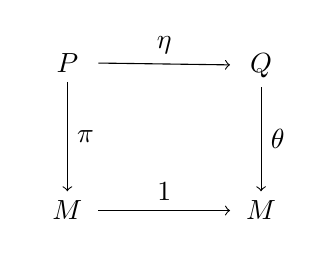
\begin{tikzpicture}
  \matrix (m) [matrix of math nodes, row sep=3.8em, column sep=4.8em, minimum width=2.2em]
  {
P & Q \\
M & M \\
};
  \path[->]
  (m-1-1) edge node [auto] {$\eta$} (m-1-2)
          edge node [auto] {$\pi$} (m-2-1)
  (m-1-2) edge node [auto] {$\theta$} (m-2-2)
  (m-2-1) edge node [auto] {$1$} (m-2-2)
  ;
\end{tikzpicture} & \quad \quad \, 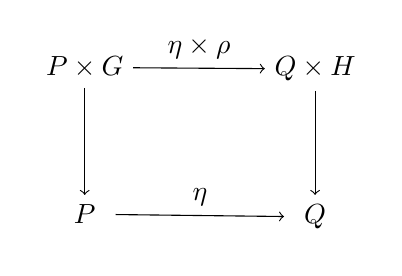
\begin{tikzpicture}
  \matrix (m) [matrix of math nodes, row sep=3.8em, column sep=4.8em, minimum width=2.2em]
  {
P\times G & Q\times H \\
P & Q \\
};
  \path[->]
  (m-1-1) edge node [auto] {$\eta \times \rho $} (m-1-2)
          edge node [auto] {$$} (m-2-1)
  (m-1-2) edge node [auto] {$$} (m-2-2)
  (m-2-1) edge node [auto] {$\eta$} (m-2-2)
  ;
\end{tikzpicture} \\
\pi(p) = \theta(\eta p) \quad \quad \, & \quad \quad \, \eta(pg) = (\eta p)(\rho g)
\end{aligned}
\]
\end{enumerate}

\end{definition}

\begin{definition}
Lee  defines the \textbf{principal $G$-bundle morphism} on pp. 298 of Lee (2009)\cite{JLee2009} as a pair $(\widetilde{f}, f)$ 
\[
(P_G, \pi, M_1) \xrightarrow{ (\widetilde{f},f) } (Q_G, \theta, M_2)
\]

s.t.
\begin{enumerate}
\item smooth $f : M_1 \to M_2$
\item $P \xrightarrow{ \widetilde{f}} Q$ morphism s.t.
\[
\begin{aligned} 
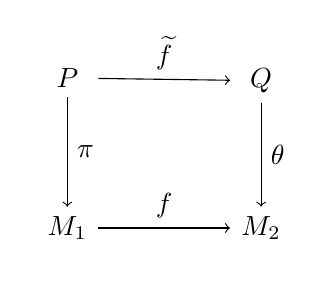
\begin{tikzpicture}
  \matrix (m) [matrix of math nodes, row sep=3.8em, column sep=4.8em, minimum width=2.2em]
  {
P & Q \\
M_1 & M_2 \\
};
  \path[->]
  (m-1-1) edge node [auto] {$\widetilde{f}$} (m-1-2)
          edge node [auto] {$\pi$} (m-2-1)
  (m-1-2) edge node [auto] {$\theta$} (m-2-2)
  (m-2-1) edge node [auto] {$f$} (m-2-2)
  ;
\end{tikzpicture} & \quad \quad \, 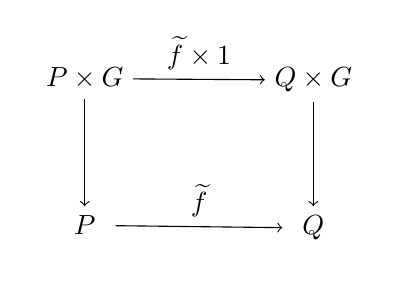
\begin{tikzpicture}
  \matrix (m) [matrix of math nodes, row sep=3.8em, column sep=4.8em, minimum width=2.2em]
  {
P\times G & Q\times G \\
P & Q \\
};
  \path[->]
  (m-1-1) edge node [auto] {$ \widetilde{f}\times 1 $} (m-1-2)
          edge node [auto] {$$} (m-2-1)
  (m-1-2) edge node [auto] {$$} (m-2-2)
  (m-2-1) edge node [auto] {$\widetilde{f}$} (m-2-2)
  ;
\end{tikzpicture} \\
f(\pi(p)) = \theta(\widetilde{f}(p)) \quad \quad \, & \quad \quad \, \widetilde{f}(pg) = \widetilde{f}(p)g
\end{aligned}
\]
\end{enumerate}
\end{definition}

Now \begin{tikzpicture}
  \matrix (m) [matrix of math nodes, row sep=3.8em, column sep=4.8em, minimum width=2.2em]
  {
P & Q \\
M &  \\
};
  \path[->]
  (m-1-1) edge node [auto] {$ \widetilde{f} $} (m-1-2)
          edge node [auto] {$\pi$} (m-2-1)
  (m-1-2) edge node [auto] {$\theta$} (m-2-1)
  ;
\end{tikzpicture}
so that $\pi(p) = \theta(\widetilde{f}(p))$, is a \emph{bundle isomorphism} (EY : 20151008 how is $\widetilde{f} :P \to Q$ an isomorphism? And how is it a diffeomorphism when restricted to fibers?)
 
From Taubes (2011) Sec. 10.9 ``Associated vector bundles'' \cite{CTaubes2011}, 

Suppose Lie group $G$, principal $G$-bundle $\pi: P\to M$.  \\
Let representation $\rho$, $\rho: G \to GL(V)$ \\
$\exists \, $ corresponding vector bundle denoted $P\times_{\rho} V := P\times V/\sim$ where $(p,v) \sim (p g^{-1}, \rho(g)v) $ \quad \, $\forall \, g \in G$.  

\begin{tikzpicture}
  \matrix (m) [matrix of math nodes, row sep=3.8em, column sep=4.8em, minimum width=2.2em]
  {
P\times_{\rho} V   \\
M \\
};
  \path[->]
  (m-1-1) edge node [auto] {$\pi$} (m-2-1)
  ;
\end{tikzpicture}  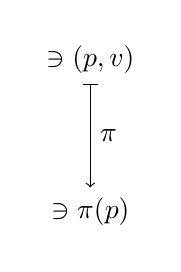
\begin{tikzpicture}
  \matrix (m) [matrix of math nodes, row sep=3.8em, column sep=4.8em, minimum width=2.2em]
  {
\ni (p,v)  \\
\ni \pi(p) \\
};
  \path[|->]
  (m-1-1) edge node [auto] {$\pi$} (m-2-1)
  ;
\end{tikzpicture}

Define \emph{zero section} $0$, to be 
\[
\begin{aligned}
  & 0 \in \Gamma(P\times_{\rho} V) \\
  & 0 = [(p,0)] \quad \, (p,0) \in P\times V
\end{aligned}
\]

Define the usual scalar multiplication by $z\in \mathbb{R} \text{ or } \mathbb{C}$, $ ( \mathbb{R} \text{ or } \mathbb{C} )\times P\times_{\rho}V \to P\times_{\rho}V$ by $(p,v) \mapsto (p,zv)$.  


Recall from the definition of a principal $G$-bundle the existence of a $G$-equivariant diffeomorphism $\varphi$: 

\begin{tikzpicture}
  \matrix (m) [matrix of math nodes, row sep=3.8em, column sep=4.8em, minimum width=2.2em]
  {
\left. P \right|_{\pi^{-1}(U)} & U\times G  \\
U \subset M & \\ 
};
  \path[->]
  (m-1-1) edge node [auto] {$\varphi$} (m-1-2)
          edge node [auto] {$\pi$} (m-2-1)
  ;
\end{tikzpicture}
i.e. $\varphi$ is $G$-equivariant diffeomorphism $\varphi : \left. P \right|_{\pi^{-1}(U)} \to U\times G$\, $\forall \, p \in M$ (that $\exists \, $ open $U \ni p$) s.t. 

if $\varphi(p) = (\pi(p),h(p))$, \, $h(p) \in G$, then $\varphi(pg^{-1}) = (\pi(p), h(p)g^{-1} )$, i.e.
\[
\text{ if } \begin{tikzpicture}
  \matrix (m) [matrix of math nodes, row sep=3.8em, column sep=4.8em, minimum width=2.2em]
  {
p & (\pi(p), h(p))   \\
\pi(p) &  \\
};
  \path[|->]
  (m-1-1) edge node [auto] {$$} (m-1-2)
          edge node [auto] {$\pi$} (m-2-1)
  ;
\end{tikzpicture} \text{ then } 
\begin{tikzpicture}
  \matrix (m) [matrix of math nodes, row sep=3.8em, column sep=4.8em, minimum width=2.2em]
  {
pg^{-1} & (\pi(p), h(p)g^{-1})   \\
\pi(p) &  \\
};
  \path[|->]
  (m-1-1) edge node [auto] {$$} (m-1-2)
          edge node [auto] {$\pi$} (m-2-1)
  ;
\end{tikzpicture}
\]
i.e. (EY : 20151015 I was wondering how best to diagram this smooth right action of $G$ by diffeomorphisms, $pg^{-1}$)

\begin{tikzpicture}
  \matrix (m) [matrix of math nodes, row sep=1.8em, column sep=4.8em, minimum width=2.2em]
  {
    G & \\
    \left. P \right|_{\pi^{-1}(U)} \times G & \\
 \left. P \right|_{\pi^{-1}(U)} & U\times G   \\
  p \in U\subset M &  \\
};
  \path[->]
  (m-2-1) edge node [auto] {$$} (m-1-1)
          edge node [auto] {$m$} (m-3-1)
  (m-3-1) edge node [auto] {$\varphi$} (m-3-2)
          edge node [auto] {$\pi$} (m-4-1)
  ;
\end{tikzpicture} \quad \quad \, \begin{tikzpicture}
  \matrix (m) [matrix of math nodes, row sep=1.8em, column sep=4.8em, minimum width=2.2em]
  {
    g & \\
    (p,g) & \\
 pg^{-1} \equiv m(p,g) & (\pi(p), h(p)g^{-1}) \\ 
\pi(p)  \\
};
  \path[|->]
  (m-2-1) edge node [auto] {$$} (m-1-1)
          edge node [auto] {$m$} (m-3-1)
  (m-3-1) edge node [auto] {$\varphi$} (m-3-2)
          edge node [auto] {$\pi$} (m-4-1)
  ;
\end{tikzpicture}

or 

\begin{tikzpicture}
  \matrix (m) [matrix of math nodes, row sep=3.8em, column sep=4.8em, minimum width=2.2em]
  {
\left. P \right|_{\pi^{-1}(U)} & U \times G   \\
p \in U \subset M  &  \\
};
  \path[->]
  (m-1-1) edge [loop above] node [auto] {$m(g)$} (m-1-1)
          edge node [auto] {$\varphi$} (m-1-2)
          edge node [auto] {$\pi$} (m-2-1)
  ;
\end{tikzpicture}
\quad \quad \, 
\begin{tikzpicture}
  \matrix (m) [matrix of math nodes, row sep=3.8em, column sep=4.8em, minimum width=2.2em]
  {
pg^{-1} & (\pi(p), h(p)g^{-1})   \\
\pi(p) &  \\
};
  \path[|->]
  (m-1-1) edge [loop above] node [auto] {$m(g)$} (m-1-1)
          edge node [auto] {$\varphi$} (m-1-2)
          edge node [auto] {$\pi$} (m-2-1)
  ;
\end{tikzpicture}



Recall $\begin{aligned} & \quad \\
  & (\varphi^V)^{-1} : U \times V \to P\times_{\rho} V \\
  & (\varphi^V)^{-1}(x,v) = [ (\varphi^{-1}(x,1),v) ]
\end{aligned}$

Then 
\[
\begin{gathered}
  \varphi^V \circ (\varphi^V)^{-1}(x,v) = \varphi^V( [(\varphi^{-1}(x,1),v)]) = \varphi^V( (\varphi^{-1}(x,1),v) ) = (x,\rho(1)v) = (x,1v) = (x,v) 
\end{gathered}
\]
Checking well-definedness (of the $\varphi^V$ operation), so given that 
\[
(\varphi^{-1}(x,1), v) \sim (\varphi^{-1}(x,1) g^{-1}, \rho(g)v) \quad \, \forall \, g\in G
\]
and so 
\[
\begin{gathered}
  \varphi^V(\varphi^{-1}(x,1)g^{-1},\rho(g)v) = (\pi(\varphi^{-1}(x,1)g^{-1}), \rho(\psi(\varphi^{-1}(x,1)g^{-1}) )\rho(g)v) = (x,\rho(\psi(\varphi^{-1}(x,1)))\rho(g^{-1})\rho(g)v)= (x,v)
\end{gathered}
\]
Thus, $\varphi^V\circ (\varphi^V)^{-1} = 1_{U\times V}$.  

Let (or recall) principal bundle isomorphisms $\begin{aligned} & \quad \\
  & \varphi_{\alpha} : \left. P \right|_{\pi^{-1}(U_{\alpha})} \to U_{\alpha} \times G \\
  & \varphi_{\beta} : \left. P \right|_{\pi^{-1}(U_{\beta})} \to U_{\beta} \times G \\
\end{aligned}$.  Then $\begin{aligned} & \quad \\
  & \varphi_{\beta} \varphi_{\alpha}^{-1} : U_{\alpha} \bigcap U_{\beta} \times G \to U_{\alpha} \bigcap U_{\beta} \times G \\
  & \varphi_{\beta} \varphi_{\alpha}^{-1} : (x,g) \mapsto (x,g_{\beta \alpha} g) \end{aligned}$ (i.e. principle $G$-bundles have principal bundle transition functions $g_{\beta\alpha}$'s).  

Then for $\begin{aligned} & \quad \\
  & \varphi^V :P\times_{\rho}V \to U\times V \\
  & \varphi^V: [(p,v)] = (p,v) \mapsto (\pi(p), \rho(\psi(p))v ) \end{aligned}$, 

\[
\begin{aligned}
  & \left. \varphi_{\alpha}^V :( P \times_{\rho} V ) \right|_{\pi^{-1}(U_{\alpha})} \to U_{\alpha} \times V \\ 
  & \left. \varphi_{\beta}^V :( P \times_{\rho} V ) \right|_{\pi^{-1}(U_{\beta})} \to U_{\beta} \times V 
\end{aligned}
 \Longrightarrow 
\begin{aligned} 
  & \varphi_{\beta}^V (\varphi_{\alpha}^V)^{-1} : U_{\alpha} \bigcap U_{\beta} \times V \to U_{\alpha} \bigcap U_{\beta} \times V \\ 
  &  \varphi_{\beta}^V (\varphi_{\alpha}^V)^{-1}: (x,v) \mapsto (x,\rho(g_{\beta \alpha}) v)
\end{aligned}
\]
So for our vector bundle $P\times_{\rho}V$, we have smooth, invertible ``transition'' maps $\varphi_{\beta}^V (\varphi_{\alpha}^V)^{-1}$ defined as immediately above.  

Thus

\begin{proposition}
  Given principle $G$-bundle $\pi: P \to M$, Lie group $G$, representation $\rho$, $\rho:G \to GL(V)$, then $\exists \, $ (an associated) vector bundle $P\times_{\rho}V := P\times V/\sim$ where $(p,v) \sim (pg^{-1},\rho(g)v)$ \, $\forall \, g \in G$ s.t. for this vector bundle $P\times_{\rho}V$, we have local trivialization $\varphi^V$, $P\times_{\rho}V \xrightarrow{ \varphi^V} U\times V$, defined as such:

For principal $G$-bundle $\pi : P \to M$, 

\begin{tikzpicture}
  \matrix (m) [matrix of math nodes, row sep=3.8em, column sep=4.8em, minimum width=2.2em]
  {
P \\ 
M \\
};
  \path[->]
  (m-1-1) edge node [auto] {$\pi$} (m-2-1)
  ;
\end{tikzpicture}
 \, \begin{tikzpicture}
  \matrix (m) [matrix of math nodes, row sep=3.8em, column sep=4.8em, minimum width=2.2em]
  {
\supset \left. P \right|_{\pi^{-1}(U)} & U\times G & G \\ 
\supset U \ni x & & \\
};
  \path[->]
  (m-1-1) edge node [auto] {$\varphi$} (m-1-2)
          edge [bend left=30] node [auto] {$\psi$} (m-1-3)
  (m-1-2) edge node [auto] {$$} (m-1-3)
          edge node [auto] {$$} (m-2-1) 
  (m-2-1) edge node [auto] {$\pi^{-1}$} (m-1-1)    
  ;
\end{tikzpicture} define 
\[
\begin{aligned}
  & \varphi^V : P\times_{\rho} V \to U\times V \\ 
  & [(p,v)] =(p,v) \mapsto (\pi(p),\rho(\psi(p))v)
\end{aligned}
\]
and 
\[
\begin{aligned}
  & (\varphi^V)^{-1} : U\times V \to P\times_{\rho}V \\ 
  & (x,v) \mapsto [(\varphi^{-1}(x,1),v) ]
\end{aligned}
\]
and define the transition functions for our (associated) vector bundle $P\times_{\rho}V$ as such: for principal bundle isomorphisms $\begin{aligned} & \quad \\
  & \varphi_{\alpha} : \left. P \right|_{\pi^{-1}(U_{\alpha})} \to U_{\alpha} \times G \\
  & \varphi_{\beta} : \left. P \right|_{\pi^{-1}(U_{\beta})} \to U_{\beta} \times G \\
\end{aligned}$, then resulting principal bundle transition functions are such: $\begin{aligned} & \quad \\
  & \varphi_{\beta} \varphi_{\alpha}^{-1} : U_{\alpha} \bigcap U_{\beta} \times G \to U_{\alpha} \bigcap U_{\beta} \times G \\
  & \varphi_{\beta} \varphi_{\alpha}^{-1} : (x,g) \mapsto (x,g_{\beta \alpha} g) \end{aligned}$, and so we have transition functions for our (associated) vector bundle 

\[
\begin{aligned}
  & \left. \varphi_{\alpha}^V :( P \times_{\rho} V ) \right|_{\pi^{-1}(U_{\alpha})} \to U_{\alpha} \times V \\ 
  & \left. \varphi_{\beta}^V :( P \times_{\rho} V ) \right|_{\pi^{-1}(U_{\beta})} \to U_{\beta} \times V 
\end{aligned}
 \Longrightarrow 
\begin{aligned} 
  & \varphi_{\beta}^V (\varphi_{\alpha}^V)^{-1} : U_{\alpha} \bigcap U_{\beta} \times V \to U_{\alpha} \bigcap U_{\beta} \times V \\ 
  &  \varphi_{\beta}^V (\varphi_{\alpha}^V)^{-1}: (x,v) \mapsto (x,\rho(g_{\beta \alpha}) v)
\end{aligned}
\]

\end{proposition}


\begin{claim}
  If smooth map $\sigma^P:P \to V$ s.t. $\sigma^P(pg^{-1}) = \rho(g)\sigma^P(p)$, $\exists \, $ section $\sigma \in \Gamma(P\times_{\rho}V)$, defined as 
\[
\sigma(x) = [(p,\sigma^P(p))] \text{ s.t. } \pi(p) = x \, x \in M
\]
  If given section $\sigma \in \Gamma(P\times_{\rho}V)$, $\exists \, $ smooth map $\sigma^P:P\to V$ s.t. $\sigma^P(pg^{-1}) = \rho(g)\sigma^P(p)$
\end{claim}
cf. Taubes (2001), Subsec. 11.4.1 Part 1

\begin{proof}
  If given $\sigma^P: P \to V$ s.t. $\sigma^P(pg^{-1}) = \rho(g)\sigma^P(p)$, let 
\[
\sigma(x) = [(p,\sigma^P(p))] \text{ s.t. } \pi(p) = x
\]
Indeed, checking well-definedness for $(p,\sigma^P(p)) \sim (pg^{-1}, \rho(g)\sigma^P(p))$, 
\[
(pg^{-1}, \rho(g)\sigma^P(p)) = (pg^{-1}, \sigma^P(pg^{-1})) = \sigma(x)
\]
since $\pi(pg^{-1})=x$.  Since $\pi(pg^{-1})=x$ \, $\forall \, g\in G$, then indeed this section $\sigma \in \Gamma(P\times_{\rho}V)$ is well-defined.  
  
\end{proof}

\begin{proposition}[cf. Taubes (2001) Subsection 11.4.3 \cite{CTaubes2011}]
$\forall \, $ principal $G$-bundle $\pi:P \to M$, $\exists \, $ short exact sequence of vector bundle homomorphims
\begin{equation}
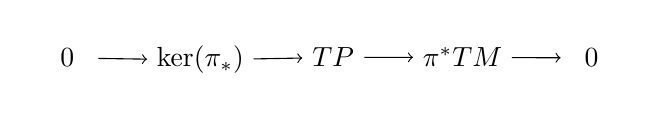
\begin{tikzpicture}
  \matrix (m) [matrix of math nodes, row sep=1.8em, column sep=1.8em, minimum width=2.2em]
  {
0 & \text{ker}{ (\pi_* )}  & TP & \pi^*TM & 0 \\
};
  \path[->]
  (m-1-1) edge node [auto] {$$} (m-1-2)
  (m-1-2) edge node [auto] {$$} (m-1-3)
  (m-1-3) edge node [auto] {$$} (m-1-4)    
  (m-1-4) edge node [auto] {$$} (m-1-5)    
  ;
\end{tikzpicture} 
\end{equation}
s.t. 

$\pi_* : TP \to TM$ and so \\
$\text{ker}\pi_* \subset TP$

and so with arrows meaning, as follows:

$\text{ker}{\pi_*} \xrightarrow{ \mathbf{i}} TP$, inclusion $\mathbf{i}$, 

$\begin{aligned} & TP \to \pi^*TM \\
  & v\in TP \mapsto (\pi(p), \pi_*v) \in \pi^*TM \subset P \times TM \end{aligned}$



\end{proposition}

Recall (smooth, right) action of $G$ on $P$, $\begin{aligned} & \quad \\
   m(g) \equiv m_g & : P \to P \\
  m_g & : p\mapsto pg^{-1} \end{aligned}$ \quad \, $\forall \, g \in G$.  Then $\begin{aligned} & \quad \\
  & (m_g)_* : TP \to TP \\
  & (m_g)_*:v_p \mapsto v_{pg^{-1}}\end{aligned}$.  

If $v\in TP$, $v\in \text{ker}\pi_*$, $(m_g)_*v \in \text{ker}\pi_*$ since $\pi_*((m_g)_*v) = (\pi \circ m_g)_*v = (\pi_*)v = 0$ \\
(for $\pi\circ m_g(p) = \pi(pg^{-1}) = \pi(p)$, so $\pi \circ m_g = \pi$)


There are many parts of this sequence to parse out and understand.  

Begin with 
\[
\pi_* : TP \to TM
\]
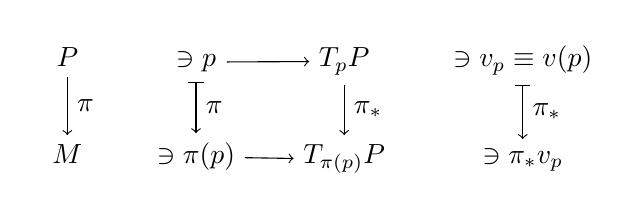
\begin{tikzpicture}
  \matrix (m) [matrix of math nodes, row sep=1.8em, column sep=1.8em, minimum width=2.2em]
  {
    P & \ni p      & T_pP        & \ni v_p \equiv v(p) \\
    M & \ni \pi(p) & T_{\pi(p)}P & \ni \pi_*v_p \\
};
  \path[->]
  (m-1-1) edge node [auto] {$\pi$} (m-2-1)
  (m-1-2) edge node [auto] {$$} (m-1-3)
  (m-1-3) edge node [auto] {$\pi_*$} (m-2-3)    
  (m-2-2) edge node [auto] {$$} (m-2-3)    
  ;
  \path[|->]
  (m-1-2) edge node [auto] {$\pi$} (m-2-2)
  (m-1-4) edge node [auto] {$\pi_*$} (m-2-4)
;
\end{tikzpicture} 

$\text{ker}{\pi_*}$ \emph{is} the so-called vertical bundle of $\pi_* : TP \to TM$ \footnote{``Vertical bundle'', \emph{Wikipedia} \url{https://en.wikipedia.org/wiki/Vertical_bundle}}.

\begin{claim}
This sequence
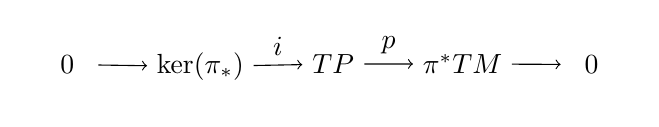
\begin{tikzpicture}
  \matrix (m) [matrix of math nodes, row sep=1.8em, column sep=1.8em, minimum width=2.2em]
  {
0 & \text{ker}{ (\pi_* )}  & TP & \pi^*TM & 0 \\
};
  \path[->]
  (m-1-1) edge node [auto] {$$} (m-1-2)
  (m-1-2) edge node [auto] {$i$} (m-1-3)
  (m-1-3) edge node [auto] {$p$} (m-1-4)    
  (m-1-4) edge node [auto] {$$} (m-1-5)    
  ;
\end{tikzpicture} 
is a short exact sequence.
\end{claim}

\begin{proof}
  Consider $i : \text{ker}(\pi_*) \to TP$ (inclusion) \\
$i(a) = i(a')$, $a, a' \in \text{ker}\pi_*$.  Then $a=a'$.  Inclusion $i$ is injective.  So $0 \to \text{ker}(\pi_*) \to TP$ exact.  (this is shown mathematically in Rotman, or my notes on Rotman, or in your favorite abstract algebra book or notes) 

EY : 20151017 weblinks roundup:

This showed that vector fields are isomorphic to derivations, and explicitly gives the construction of the isomorphism: 1300Y Geometry and Topology \url{http://www.math.toronto.edu/mgualt/MAT1300/week9.pdf}

This clarifies Taubes, 11.4.4 Part 3-4 \url{http://xwww.uni-math.gwdg.de/upmeier/notes/connections.pdf}

Since the Snake Lemma and 5-lemma are needed to show, in a civilized manner, the splitting lemma, could we use the Snake Lemma and 5-lemma for connections on a principal-G bundle? \url{http://www.mathematik.uni-kl.de/~gathmann/class/commalg-2013/chapter-4.pdf}

\end{proof}

\part{Gauge Theory}

The story of Gauge Theory in Physics is a beautiful story - it is the triumph of geometry in physical theories of matter.  

\section{Electromagnetism}

\begin{description}
\item Electromagnetism
\item Maxwell's Equations
\end{description}

From ``Rewriting Maxwell's Equations'' of Baez and Muniain (1994) \cite{JBaezJMuniain1994}:  


\[
\begin{aligned}
  & *F_+ = \frac{1}{2} \left[ i F_+ -iF_- + i(F_+ + F_-) \right] = iF_+ \text{ i.e. self dual }
  & *F_- = \frac{1}{2} \left[ i F_+ -iF_- - iF_+ -i F_-  \right] = -iF_- \text{ i.e. anti-self dual }
\end{aligned}
\]


So if $F \in \Omega^p(M)$ ($F$ self dual or anti self dual), if $dF=0$, $d*F =0$, since $d*F = \begin{cases} d( \pm F) = \pm dF = 0 \\
  d(\pm iF) = \pm i dF = 0\end{cases}$

Consider $\begin{aligned} & \quad \\
  & \Delta : \Omega^p(M) \to \Omega^p(M) \\
  & \Delta = (\delta +d)^2 = \delta d + d\delta \end{aligned}$

\[
\Delta F = \delta dF + d\delta F = 0 + d (-*d*) F = -dJ 
\]
\[
\begin{aligned}
   J & = j - \rho dt \\ 
   dJ & = \frac{ \partial j_j}{ \partial x^{\mu} } dx^{\mu} \wedge dx^j - \frac{ \partial \rho}{ \partial x^i} dx^i \wedge dt
\end{aligned}
\]


Note that for $d^2 =0$, $\delta^2=0$ (as seen with this example of Maxwell's equations, for $F$), $\delta = (-1)^{n(p+1)+1} *d* = -*d*$ (especially if $n$ even), 

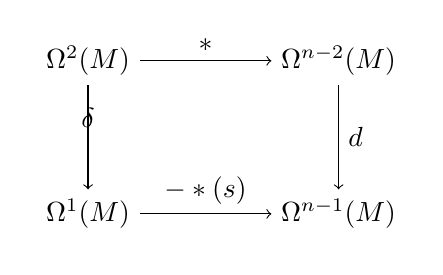
\begin{tikzpicture}
  \matrix (m) [matrix of math nodes, row sep=3.8em, column sep=4.8em, minimum width=2.2em]
  {
    \Omega^2(M) & \Omega^{n-2}(M) \\
    \Omega^1(M) & \Omega^{n-1}(M)   \\
};
  \path[->]
  (m-1-1) edge node [above] {$*$} (m-1-2)
          edge node [above] {$\delta$} (m-2-1)
  (m-1-2) edge node [auto]  {$d$} (m-2-2)
  (m-2-1) edge node [auto]  {$-*(s)$} (m-2-2)
  ;
\end{tikzpicture} \quad \quad \, 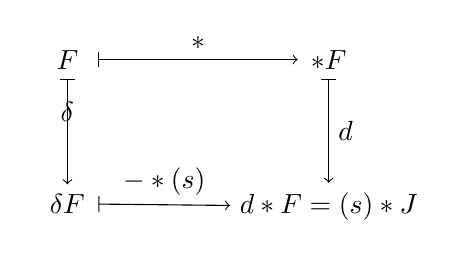
\begin{tikzpicture}
  \matrix (m) [matrix of math nodes, row sep=3.8em, column sep=4.8em, minimum width=2.2em]
  {
    F & *F \\
    \delta F & d*F = (s)*J \\
};
  \path[|->]
  (m-1-1) edge node [above] {$*$} (m-1-2)
          edge node [above] {$\delta$} (m-2-1)
  (m-1-2) edge node [auto]  {$d$} (m-2-2)
  (m-2-1) edge node [auto]  {$-*(s)$} (m-2-2)
  ;
\end{tikzpicture}


\[
\begin{aligned}
  & F \in \Omega^2(M) \\ 
  & F = \frac{1}{2} F_{\mu \nu} dx^{\mu} \wedge dx^{\nu}
\end{aligned} \quad \quad \, 
\begin{aligned}
  & *F \in \Omega^{n-2}(M) \\ 
  & *F = \frac{\sqrt{g}}{ (n-2)!} \frac{1}{2} F_{\mu \nu} g^{\mu \mu'} g^{\nu \nu'} \epsilon_{\mu' \nu' \rho \sigma } dx^{\rho} \wedge dx^{\nu} 
\end{aligned}
\]

\[
\begin{aligned}
  F & = B + E \wedge dt = \frac{B_{ij}}{2} dx^i \wedge dx^j + E_i dx^i \wedge dt \\ 
*F & = \frac{ \sqrt{g}}{(n-2)!} \frac{B_{ij}}{2} g^{i \mu } g^{j \nu} \epsilon_{\mu \nu \rho \sigma } dx^{\rho} \wedge dx^{\sigma} +   \frac{ \sqrt{g}}{ (n-2)!} E_i g^{i\mu} g^{0\nu} \epsilon_{\mu \nu \rho \sigma} dx^{\rho} \wedge dx^{\sigma}
\end{aligned}
\]

If $M = \mathbb{R}\times N$, 
\[
\begin{gathered}
  B_{ij} g^{il}g^{jm} \epsilon_{lm\rho \sigma} dx^{\rho} \wedge dx^{\sigma} = B_{ij} g^{il}g^{jn} (\epsilon_{lmn\sigma} dx^n \wedge dx^{\sigma} + \epsilon_{lm0\sigma} dx^0 \wedge dx^{\sigma} ) = \\
  = B_{ij} g^{il} g^{jm} (\epsilon_{lmn0} dx^n \wedge dt + \epsilon_{lmn} dx^n \wedge dt) = 2B_{ij} g^{il} g^{jm} \epsilon_{lmn} dx^n \wedge dt
\end{gathered}
\]

Noting that 
\[
\epsilon_{lmn} B_{ij} g^{il} g^{jm} = \epsilon_{lmn} \epsilon_{ijk} B^k g^{il} g^{jm} = 2B^n
\]


If $g= \left( \begin{matrix} -1  & & & \\
  & 1 & & \\
  &  & 1 & \\
  & & & 1 \end{matrix} \right)$ and $M = \mathbb{R} \times N$, 
\[
\begin{aligned}
  *F & = \frac{1}{ (n-2)!} \left[ \frac{B_{ij}}{2} g^{il }g^{jm} \epsilon_{lmn0} dx^n \wedge dt + -E_i g^{il} \epsilon_{l0mn} dx^m \wedge dx^n \right] = \frac{1}{(n-2)!} \left[ -\epsilon_{lmn} g^{li} E_i dx^m \wedge dx^n + (-\epsilon_{lmn})B_{ij} g^{il} g^{jm} dx^n \wedge dt \right] = \\
  & = \frac{1}{(n-2)!} \left[ -E_i g^{il} \epsilon_{lmn} dx^m \wedge dx^n + (-B_{ij}) g^{il} g^{jm} \epsilon_{lmn} dx^n \wedge dt \right] = \vec{*} E - \vec{*}B \wedge dt
\end{aligned}
\]

Indeed, in general, for $M = \mathbb{R}\times N$, 
\[
\begin{gathered}
  *F = \frac{ \sqrt{g}}{ (n-2)!} B_{ij} g^{il}g^{jm} \epsilon_{lmn0} dx^n \wedge dt + \frac{\sqrt{g}}{(n-2)!} E_i g^{il} (-1) \epsilon_{l0mn} dx^m \wedge dx^n = \\
  =  \frac{\sqrt{g}}{ (n-2)!}(-1)E_i g^{il} (-\epsilon_{0lmn}) dx^m \wedge dx^n + \frac{\sqrt{g}}{(n-2)!} \epsilon_{ijk} B^k g^{il} g^{jm} (-\epsilon_{lmn})dx^n \wedge dt
\end{gathered}
\]
If $g^{il}= \delta^{il}$, then applying $\epsilon_{jmn}\epsilon^{imn} = 2\delta^i_j$, and $n=4$
\[
*F = \vec{*}E + \vec{*}B \wedge dt
\]

$*F = iF$ (self-dual) if 
\[
\begin{aligned}
  & \vec{*} E= iB \\ 
  & \vec{*} B= -i E
\end{aligned}
\]

And so 
\[
\begin{gathered}
  E = E_i dx^i \\ 
  \vec{*} E = \frac{ \sqrt{g}}{ (d-1)!} E_i g^{il} \epsilon_{lmn} dx^m \wedge dx^n \Longrightarrow -i \vec{*} E = \frac{-i\sqrt{g}}{ (d-1)!} E_i g^{il} \epsilon_{lmn} dx^m \wedge dx^n \\ 
  B = \frac{1}{2} B_{mn} dx^m \wedge dx^n = \frac{1}{2} \epsilon_{mnl} B^l dx^m \wedge dx^n 
\end{gathered} \Longrightarrow \frac{1}{2} B^l = \frac{-i \sqrt{g}}{ (d-1)!} E_i g^{il} \text{ or } B^k = -i \sqrt{g} E_i g^{ik}
\]


Assume $F$ self-dual ($*F = iF$) and $E(x) = E_i e^{ikx} dx^i$, $k \in (\mathbb{R}^4)^*$, $x\in \mathbb{R}^4 = M$, $k$ fixed covector called \textbf{energy-momentum}, s.t. 
\[
k_{\mu} x^{\mu} = kx
\]
$B= -i \vec{*} E$




\section{Chern-Simons Theory}

From Baez and Muniain (1994) \cite{JBaezJMuniain1994}: 




\part{Polynomials}

\section{(Software) Packages}

This link \href{http://www.mat.univie.ac.at/~slc/divers/software.html}{Combinatorial Software and Databases} has a list of (possibly) useful implementations of the Gosper-Zeilberger Algorithm.  There is 
\begin{itemize}
\item \href{http://www.math.rutgers.edu/~zeilberg/tokhniot/EKHAD}{EKHAD}: written in Maple by Doron Zeilberger, is an implementation of the Gosper-Zeilberger algorithm.
\item \href{http://www.math.rutgers.edu/~zeilberg/tokhniot/qEKHAD}: written in Maple by Doron Zeilberger, is an implementation of the q-Zeilberger algorithm.  Also at \href{http://www.math.rutgers.edu/~zeilberg/programsAB.html}{Rutgers, Packages Accompanying or Related to A=B}
\item \href{http://www.risc.uni-linz.ac.at/research/combinat/risc/software/Zeilberger/}{Zeilberger}:written in Maxima by Fabrizio Caruso, is an implementation of the Gosper-Zeilberger algorithm.
\end{itemize}

Tom Koornwinder had a paper \href{https://staff.fnwi.uva.nl/t.h.koornwinder/art/1993/zeilbalgo.pdf}{On Zeilberger’s algorithm and its $q$-analogue: a rigorous description} that explicitly and very lucidly reviews Zeilberger's algorithm, but I cannot find his accompanying Maple software (links don't work).  

I will focus on looking at Caruso's package because the source code is available and I had emailed Paule and the source code for Mathematica implementations are not available, understandably from their particular policies on distribution.

Wilf and Zeilberger (1992) has a good introduction to hypergeometric polynomials and its significance \cite{HWilfDZeilberger1992}.  In the immediate sections, I will recap, summarize, and copy (or state) some definitions and results from  Wilf and Zeilberger (1992), and show (some of its) direct implementations in Sage Math and sympy.    

Starting from pp. 586 of Wilf and Zeilberger (1992) \cite{HWilfDZeilberger1992},  \\
Consider 
\[
(c)_n := (1-c)(1-cq) \dots (1-cq^{n-1})
\]
Let $c=q$.  Then
\[
(q)_n = (1-q)(1-q^2)\dots (1-q^n)
\]
Define $f(n):= (c)_n$.  Notice that 
\[
\frac{f(n+1)}{f(n)} = 1 - cq^n
\]
This is the simplest nonzero rational function in $q^n$.  

Let $f(x):=(x)_{\infty}$.  $\frac{f(qx)}{f(x)} = \frac{(qx)_{\infty} }{(x)_{\infty}} = \frac{1}{1-x}$.  

Note that 
\[
\begin{gathered}
  \frac{1}{1-x} = \sum_{j=0}^{\infty}x^j \\ 
  \begin{aligned}
    & (x)_{\infty} = (1-x)(1-xq) \dots (1-xq^{n-1}) \dots \\ 
    & (qx)_{\infty} = (1-qx)(1-q^2x)\dots (1-xq^n) \dots
\end{aligned}
\end{gathered}
\]
Also note that 
\[
(q)_k  =\frac{ (q)_{\infty} }{ (q^{k+1})_{\infty}} = \frac{(1-q)(1-q^2) \dots (1-q^n) }{ (1-q^{k+1})(1-q^{k+2})\dots }
\]
Introduce dilation operator $\forall \, x \in \mathbb{F}$, $Q_xf(x,\mathbf{y}) := f(qx,\mathbf{y})$

$q$-derivative $D_x^{(q)}$
\[
D_x^{(q)}f(x,\mathbf{y}) = \frac{f(qx,\mathbf{y}) - f(x,\mathbf{y}) }{(q-1)x} = \frac{(Q_x -1)f(x,\mathbf{y})}{(x(q-1) ) }
\]

Notice that 
\[
\lim_{q\to 1} D^{(q)}_xf(x,\mathbf{y}) = D_x f
\]

\begin{definition}
  $q$-hypergeometric,
\[
F(k_1 \dots k_r, y_1 \dots y_s) \equiv F(\mathbf{k},\mathbf{y})
\]
$k_1 \dots k_r \in \mathbb{Z}$ (discrete), $y_1 \dots y_s$ cont. ($y_1 \dots y_s \in \mathbb{F} \in \lbrace \mathbb{R}, \mathbb{C} \rbrace$) \emph{$q$-hypergeometric} \\

if $\begin{aligned} & \quad \\ 
  & \forall \,  \text{ (discrete) } \, k_i \, , \, (E_{k_i}F)/F \\ 
  & \forall \, \text{ (cont.) } \, y_j \, , \, (Q_{y_j}F)/F \end{aligned}$ rational functions of $(q^{k_1} \dots q^{k_r}, y_1 \dots y_s)$ and possible other constnat parameters, including $q$.  
\end{definition}

\subsubsection{Examples}
\begin{enumerate}
\item  Polynomials $P(q^{k_1} \dots q^{k_r}, y_1 \dots y_n)$.  Indeed, 
\[
\begin{gathered}
  (E_{k_i}P)/P = \frac{ P(q^{k_1} \dots q^{k_i +1} \dots q^{k_r}, \mathbf{y}) }{ P(q^{k_1} \dots q^{k_r}, \mathbf{y}) } \\
  (Q_{y_j}P)/P = \frac{ P(q^{k_1} \dots q^{k_r}, y_1 \dots qy_j \dots y_n ) }{ P(q^{k_1} \dots q^{k_r},y_1 \dots y_n ) } \end{gathered}
\]
\item \[
(cy_1^{\alpha_1} \dots y_s^{\alpha_s}, q^{\beta_1 k_1} \dots q^{\beta_r k_r})^{\gamma}_{\infty}
\]cf. (qPH-II) of Wilf and Zeilberger (1992) \cite{HWilfDZeilberger1992} EY : 20160105 I don't understand the upper and lower exponent notation of $()^{\gamma}_{\infty}$, i.e. what is $\gamma$ and $\infty$ in this case?
\item $q^{\sum_{i,j} a_{i,j} k_i k_j + \sum_i b_i k_i }$ \quad \, $a_{i,j},b_i \in \mathbb{Z}$ or $\lbrace \pm \frac{1}{2}, \pm \frac{3}{2} , \dots \rbrace$.  Indeed
\[
\xrightarrow{ E_{k_i} } q^{\sum_{i,j} q_{i,j} k_i k_j + \sum_i b_i k_i } q^{\sum_{i,j}a_{i,j}k_j + b_i}
\]
\item $z_1^{k_1} \dots z_r^{k_r}$.  Indeed,
\[
\xrightarrow{E_{k_i}} z_1^{k_1} \dots z_r^{k_r} \cdot z_i
\]
\end{enumerate}

\begin{definition}
$F(k_1\dots k_r,y_1 \dots y_s)$, (discrete) $k_1 \dots k_r \in \mathbb{Z}$, (cont.) $y_1 \dots y_r \in \mathbb{F} \in \lbrace \mathbb{R}, \mathbb{C} \rbrace$, \emph{$q$-proper-hypergeometric} \\
if $F$ has form $F = P(q^{k_1} \dots q^{k_r}, y_1 \dots y_s) \cdot q^{ \sum_{i,j} a-{i,j}k_ik_j + \sum_i b_i k_i } \cdot z_1^{k_1} \dots z_r^{k_r} \cdot \text{ finite number of } (cy_1^{\alpha_1} \dots y_s^{\alpha_s} q^{\beta_1 k_1} \dots q^{\beta_r k_r } )_{\infty}^{\gamma}$
\end{definition}

\begin{lemma}[$q$-fundamental lemma]
$\forall \, $ $q$-proper-hypergeometric $F(x_1\dots x_n,a_1 \dots a_m)$ and $\forall \, $ cont. $x_i$, $\forall \, $ (discrete) $a_j$, $\exists \, $ nonzero linear recurrence-$q$-differential operators

\[
P_i(x_i; Q_{x_1} \dots Q_{x_n}; E_{a_1} \dots E_{a_m} ) \text{ and respectively } C_j(q^{a_j}; Q_{x_1} \dots Q_{x_n} ; E_{a_1} \dots E_{a_m} )
\]
annihilating $F$, i.e. $\begin{aligned} & \quad \\
  & P_iF = 0  \\
  & C_jF =0 \end{aligned}$
\end{lemma}

Let $x=q^k$
\[
\begin{aligned}
  & (cq^k)_{\infty} = \frac{(c)_{\infty}}{(c)_k} = \frac{(1-c)(1-cq) \dots }{ (1-c)(1-cq) \dots (1-cq^{k-1} )} = (1-cq^k)(1-cq^{k+1}) \dots \\ 
  & (cx)_{\infty} = \frac{(c)_{\infty}}{(c)_k} = (1-cq)(1-cxq) \dots 
\end{aligned}
\]
Consider these transformations or mappings:
\[
\begin{gathered}
  F(x_1 \dots x_n, a_1 \dots a_m) \xrightarrow{ x=q^k} F(q^{k_1} \dots q^{k_n}, a_1 \dots a_m) \\ 
  Q_{x_i} F = F(x_1 \dots qx_i \dots x_n, \mathbf{a}) = F(q^{k_1} \dots q^{(1+k_i)} \dots q^{k_n}, \mathbf{a}) = E_{k_i}F
\end{gathered}
\]
$E_kq^k = qq^k E_k$ is ``isomorphic'' to $Q_xx = qxQ_x$

Now for $\frac{(c)_{\infty}}{(cx)_{\infty}} $ substitute $(c)_k$.  
\[
\frac{(c)_{\infty}}{(cx)_{\infty}} = \frac{(1-c)(1-cq) \dots }{ (1-cx)(1-cxq) \dots } \xrightarrow{ x=q^k} (1-c)(1-cq) \dots (1-cq^{k-1})
\]

\subsection{The fundamental theorem of hypergeometric summation/integration}

cf. Sec. 2. ``The fundamental theorem of hypergeometric summation/integration'' of Wilf and Zeilberger (1992) \cite{HWilfDZeilberger1992}.  

\begin{definition}
  $F(k_1 \dots k_r, y_1 \dots y_s) \equiv F(\mathbf{k}, \mathbf{y})$ vanishes at infinity if $\forall \, k_i, y_j$,
\[
\begin{gathered}
  \lim_{|k_i|\to \infty} F(\mathbf{k},\mathbf{y}) =0 \\
  \lim_{|y_j|\to \infty} F(\mathbf{k},\mathbf{y}) = 0 
\end{gathered}
\]
\end{definition}

\begin{definition}
  integral-sum
\[
\begin{gathered}
  g(n,x) := \sum_k \int_y F(n,k,x,y) dy \qquad \text{ (general-integral-sum) }
\end{gathered}
\]
is pointwise trivially evaluable, if $\forall \, $ given $\mathbf{n}, \mathbf{x}$, $\exists \, $ algorithm to evaluate it.  

e.g. for pure sums that are terminating, 
\[
g(\mathbf{n}) := \sum_{\mathbf{k}} F(n,\mathbf{k}) \qquad \text{ (general-sum) }
\]
sum is finite $\forall \, \mathbf{n}$ since $F(\mathbf{n},\cdot)$ has finite support.  
\end{definition}

\subsubsection{The fundamental Theorem of hypergeometric summation-integration}

\begin{theorem}[The fundamental theorem]
  Let $\Delta_{k_i} \equiv \text{ forward difference operator in $k_i$ }$; \, $\Delta_{k_i} := (K_i -1)$.  

Let $\begin{aligned} & \quad \\
  & F(n,k_1 \dots k_r, y_1 \dots y_s) \\ 
  & F(x,k_1 \dots k_r, y_1 \dots y_s) 
\end{aligned}$ be hypergeometric (holonomic) (both hold if proper-hypergeometric) in $\begin{aligned} & \quad \\
  & (\mathbf{k},\mathbf{y}) \text{ and } n \\
  & (\mathbf{k}, \mathbf{y}) \text{ and } x \end{aligned}$

where $\begin{aligned} & \quad \\
  & \text{ discrete } n, \mathbf{k} \\
  & \text{ cont. } x, \mathbf{y} \end{aligned}$

Then $\begin{aligned} & \quad  \\
  & \exists \, \text{ linear ordinary recurrence operator } \\
  & \exists \, \text{ linear differential operator } \end{aligned}$ with polynomial coefficients $\begin{aligned} & \quad \\
  & P(N,n) \\
  & P(D_x,x) \end{aligned}$

and rational functions $R_1 \dots R_r, S_1 \dots S_s$ s.t. 

\begin{equation}
\begin{aligned}
  & P(N,n)F = \sum_{i=1}^r \Delta_{k_i}(R_i, F) + \sum_{j=1}^s D_{y_j} (S_jF) \\ 
  & P(D_x,x)F = \sum_{i=1}^r \Delta_{k_i}(R_i, F) + \sum_{j=1}^s D_{y_j} (S_jF) 
\end{aligned}
\end{equation}

If $F$ proper-hypergeometric, it's possible to find bounds for order of $P(N,n), P(D_x,x)$, and denominators $R_i,S_j$


\end{theorem}

Recall ``the fundamental lemma'', due to Bernstein, reproduced on pp. 585 of Wilf and Zeilberger (1992) \cite{HWilfDZeilberger1992}, 
\begin{lemma}[The fundamental lemma]\label{lemma:fundamentallemma}
$\forall \, $ holonomic function $F(x_1 \dots x_n, a_1 \dots a_m)$, $\forall \, $ cont. $x_i$, $\forall \, $ discrete $a_j$, $\exists \, $ non-zero linear recurrence differential operators
\[
\begin{aligned}
  & P_i(x_i;D_{x_1} \dots D_{x_n}; E_{a_1} \dots E_{a_m}) \\ 
  &  C_j(x_i;D_{x_1} \dots D_{x_n}; E_{a_1} \dots E_{a_m}) \qquad \text{ respectively }
\end{aligned}
\]
that \emph{annihilates} $F$, i.e. $PF=0$
\end{lemma}
e.g. $(D_x^2 + I)\cos{x} = 0$

\begin{proof}
  By fundamental lemma \ref{lemma:fundamentallemma}, $\exists \, $ operator(s) 
\[
\begin{aligned} 
  & A(n,E_n,E_{k_1} \dots E_{k_r}; D_{y_1} \dots D_{y_n} ) \\ 
    & A(x;E_n,E_{k_1} \dots E_{k_r}; D_{y_1} \dots D_{y_n} ) \qquad \text{ respectively }
\end{aligned}
\]
s.t. $AF=0$

It's possible to rewrite $A$ as 
\[
\begin{aligned}
& \begin{gathered}
  A(n;E_n,E_{k_1} \dots E_{k_r} ; D_{y_1} \dots D_{y_n} ) = P(n,E_n) - \sum_{i=1}^r (E_{k_i}-1)B_i(n;E_n,E_{k_1} \dots E_{k_r}, D_y \dots D_{y_n}) - \\
  - \sum_{j=1}^s D_{y_j} \overline{B}_j(n;E_n,E_{k_1} \dots E_{k_r}; D_{y_1} \dots D_{y_n}) 
\end{gathered} \\ 
  & \begin{gathered}  
      A(x;E_{k_1} \dots E_{k_r} ; D_x, D_{y_1} \dots D_{y_n} ) = P(x,D_x) - \sum_{i=1}^r (E_{k_i}-1)B_i(x;E_{k_1} \dots E_{k_r}, D_x,D_y \dots D_{y_n}) - \\
      - \sum_{j=1}^s D_{y_j} \overline{B}_j(x;E_{k_1} \dots E_{k_r}; D_x,D_{y_1} \dots D_{y_n}) \\ 
\end{gathered}
\end{aligned}
\]
\[
\begin{aligned}
  & 0 = P(n,E_n)F - \sum_{i=1}^r (E_{k_i}-1)B_i(n,E_n,E_{k_1}\dots E_{k_r};D_{y_1} \dots D_{y_n})F - \sum_{j=1}^s D_{y_j}\overline{B}_j(n,E_n,E_{k_1} \dots E_{k_i}; D_{y_1} \dots D_{y_n})F \\
  & 0 = P(x,D_x)F - \sum_{i=1}^r (E_{k_i}-1)B_iF - \sum_{j=1}^sD_{y_j}\overline{B}_jF
\end{aligned}
\]
\end{proof}
$F$ hypergeometric, s.t. $\frac{E_kF}{F}$, $\frac{D_{y_j}F}{F}$ rational functions.  By induction, $\forall \, $ ``operator monomial''
\[
\text{Mon}:= E_n^{\alpha_0} \coprod_{i=1}^r E_{k_i}^{\alpha_i} \coprod_{j=1}^s D_{y_j}^{\beta_j} \qquad \text{ (Op-Mon) }
\]
\[
\text{Mon} := D_x^{\beta_0} \coprod_{i=1}^r E_{k_i}^{\alpha_i} \coprod_{j=1}^s D_{y_j}^{\beta_j}
\]
$\frac{\text{Mon}F}{F}$ rational function. 

$\forall \, $ operator $\begin{aligned} & \quad \\
  & T(n,k_1 \dots k_r; y_1 \dots y_s; E_n, E_{k_1} \dots E_{k_r}; D_{y_1} \dots D_{y_s} ) \\ 
  & T(k_1 \dots k_r; y_1 \dots y_s; E_{k_1} \dots E_{k_r}; D_x, D_{y_1} \dots D_{y_s} ) \end{aligned}$

$\frac{TF}{F}$ rational function, since $T$ linear combination with coefficients that are polynomials in all variables, of operator monomials.  

In a sense, one could say $T$ belongs to 
\[
\begin{aligned}
  & k[n,k_1 \dots k_r;y_1 \dots y_s] \lbrace \text{ Mon } \rbrace \to \lbrace \text{ Mon } \rbrace, \qquad & k[n,k_1 \dots k_r; y_1 \dots y_s]-\text{module } \\ 
  & k[k_1 \dots k_r;x,y_1 \dots y_s] \lbrace \text{ Mon } \rbrace \to \lbrace \text{ Mon } \rbrace, \qquad & k[k_1 \dots k_r; x,y_1 \dots y_s]-\text{module } 
\end{aligned}
\]

In particular, \[
\begin{aligned}
  & B_i(F) = R_iF \\ 
  & \overline{B}_j(F) = S_jF
\end{aligned}
\]
\[
\Longrightarrow \begin{aligned}
  & 0 = P(n,E_n)F - \sum_{i=1}^r (E_{k_i}-1)R_iF - \sum_{j=1}^s D_{y_j}S_jF \\ 
  & 0 = P(x,D_x)F - \sum_{i=1}^r(E_{k_i}-1)R_iF - \sum_{j=1}^s D_{y_j}S_jF
\end{aligned}
\]

$R_i,S_j$ are certificates.  Note Gert Almkinst observed $B_i,B_j$ not necessary to be independent of $(k_1 \dots k_i; y_1 \dots y_s)$



\begin{corollary}[Fundamental corollary]
If $\begin{aligned} & \quad \\
  & F(n,\mathbf{k}, \mathbf{y}) & \text{ hypergeometric functions } \\ 
  & F(x,\mathbf{k}, \mathbf{y}) & \text{ holonomic functions }
\end{aligned}$, and vanishes at infinity, $\begin{aligned} & \quad \\
  & \forall \, \text{ fixed } n \\ 
  & \forall \, \text{ fixed} x \end{aligned}$, then
\[
\begin{aligned}
  & f(n):=\sum_k \int F(n,\mathbf{k},\mathbf{y}) d\mathbf{y} \\ 
  & f(x):=\sum_k \int F(x,\mathbf{k},\mathbf{y}) d\mathbf{y}
\end{aligned}
\]
satisfies $\begin{aligned} & \quad \\ 
  & \text{ linear recurrence equation } \\ 
  & \text{ differential equation } \end{aligned}$ with polynomial coefficients $\begin{aligned} & \quad \\
  & P(N,n)f(n) =0  \\
  & P(D_x,x)f(x) = 0\end{aligned}$
\end{corollary}

\begin{proof}
  \[
\begin{aligned}
  & \sum_{\mathbf{k}} \int d\mathbf{y} (E_{k_i} - 1) R_iF = 0 & \text{ since } \lim_{ |k_i|\to \infty} F(\mathbf{k},\mathbf{y})=0 \\ 
  & \sum_{\mathbf{k}} \int d\mathbf{y} D_{y_j}S_jF = 0 & \text{ since } \lim_{ |y_j|\to \infty} F(\mathbf{k},\mathbf{y})=0 
\end{aligned}
\]
Again, $R_i,S_j$ are called \emph{certificates}.
\end{proof}

\subsubsection{How to find $P(N,n)$ and the certificates}

cf. 2.2. How to find $P(N,n)$ and the certificates of Wilf and Zeilberger (1992) \cite{HWilfDZeilberger1992}.  

Guess the order of $P(N,n)$, say $L$ \\
\phantom{Guess } in practice, try $L =0$.  Then $L=1, \dots $
\[
P(N,n) = \sum_{i=0}^L b_i(n)N^i
\]
guess $R_i,S_j$
\[
P(N,n) = \sum_{i=1}^r \Delta_{k_i}(R_i,F)  + \sum_{j=1}^s D_{y_j}(S_jF)
\]

Reading Riese (2003) \cite{ARiese2003},

Let \\
$\mathbf{K} = \mathbb{C}(q,\tau_1 \dots \tau_m)$ denote transcendental extension of complex numbers $\mathbb{C}$ by indeterminates $q,\tau_1 \dots \tau_m$ (transcendental extension, roughly speaking, includes elements that aren't roots of polynomials over $\mathbb{C}$), \\
$\mathbf{k} \equiv (k_1 \dots k_r) \in \otimes_{i=1}^r\mathbb{Z}$ \\
polynomial in $q^n$, $q^{\mathbf{k}}$ over $\mathbf{K}$, $P(n,\mathbf{k}) \in \mathbf{K}[q^n,q^{\mathbf{k}}]$ if $\exists \, P^* \in \mathbf{K}[x_0,x_1\dots x_r]$ s.t. $P(n,\mathbf{K}) = P^*(q^n,q^{k_1} \dots q^{k_r})$ \\
$R(n,\mathbf{k})$ is a rational function in $q^n, q^{\mathbf{k}}$ over $\mathbf{K}$, $R(n,\mathbf{k}) \in \mathbf{K}(q^n,q^{\mathbf{k}})$, if $\exists \, $ rational function $R^* \in \mathbf{K}(x_0,x_1 \dots x_r)$ s.t. 
\[
R(n,\mathbf{k}) = R^*(q^n,q^{k_1} \dots q^{k_r})
\]
\begin{definition}
  $q$-hypergeometric function $F(n,\mathbf{k})$ in $n,\mathbf{k}$ over $\mathbf{K}$ if 
\[
\frac{F(n+1,\mathbf{k})}{F(n,\mathbf{k})} , \frac{F(n,k_1 \dots k_i+1 \dots k_r)}{F(n,\mathbf{k})} \in \mathbf{K}(q^n,q^{\mathbf{k}})
\]
\end{definition}
\begin{definition}
  $\mathbf{k}$-free recurrence, if $\exists \,$ finite set $S$, $S = \lbrace s | s \in \otimes{i=1}^{r+1} \mathbb{Z} \rbrace$, if $\exists \, \sigma_{i,\mathbf{j}}(n) \in \mathbf{K}[q^n]$ s.t.
\[
\sum_{(i,\mathbf{j}) \in S} \sigma_{i,\mathbf{j}}(n)F(n-i,\mathbf{k}-\mathbf{j})=0 \quad \, \forall \, (n,\mathbf{k})
\]
s.t. $F(n-i,\mathbf{k}-\mathbf{j}) , \, \forall \, (i,\mathbf{j}) \in S$ well-defined.

$S$ is called a structure set.  
\end{definition}

Thus
\begin{align}
& \sum_{(i,\mathbf{j}) \in S} \sigma_{i,\mathbf{j}}(n)F(n-i,\mathbf{k}-\mathbf{j}) = 0 =\\
& \left( \sum_{(i,\mathbf{j}) \in S}\sigma_{i,\mathbf{j}}(n) N^{-i}\mathbf{K}^{-\mathbf{j}} \right)F(n,\mathbf{k}) = 0 \xrightarrow{ 1/F} \\
  & \sum_{(i,\mathbf{j})\in S}\sigma_{i,\mathbf{j}}(n)R_{F,i,\mathbf{j}}(n,\mathbf{k}) = 0 
\end{align}
Multiplying by denominators on both sides, 
\begin{equation}
\sum_{(i,\mathbb{j})\in S}\sigma_{i,\mathbb{j}}(n) P_{F,i,\mathbb{j}}(n,\mathbb{k})=0
\end{equation}

\begin{definition}
Let $F(n,\mathbf{k})$ be $q$-proper hypergeometric, $S$ structure set.  

for fixed $s$, $(I,\mathbf{J}) \in S$ is numerator boundary pt. $\equiv (I_s^{\text{num}}, \mathbf{J}_s^{\text{num}})$ if $Ia_s + \mathbf{J} \mathbf{b}_s \geq ia_s + \mathbf{j} \mathbf{b}_s$ \quad \, $\forall \, (i,\mathbf{j}) \in S$
\end{definition}

cf. pp. 3 Eq. (1.2.15) of Gasper and Rahman (2004) \cite{GGasperMRahman2004} and pp. 4 of Riese (2003) \cite{ARiese2003}:
\begin{definition}[$q$-shifted factorial or $q$-Pochhammer symbol]
  \begin{equation}
    (a;q)_k = \begin{cases} 1 & \text{ if } k = 0 \\
      (1-a)(1-aq)\dots (1-aq^{k-1}) & \text{ if } k > 0 \\
      \frac{1}{(1-aq^{-1})(1-aq^{-2})\dots (1-aq^{-k}) } = \frac{1}{(aq^{-k}; q)_k } = \frac{ (-q/a)^kq^{\binom{k}{2}} }{ (q/a;q)_k } & \text{ if } k <0 \end{cases}
  \end{equation}
and define
\begin{equation}
  (a;q)_{\infty} = \coprod_{k=0}^{\infty}(1-aq^k)
\end{equation}
Notice that 
\begin{equation}
  \frac{ (a;q)_{\infty} }{ (q^ka;q)_{\infty} } = (a;q)_k
\end{equation}
\end{definition}

From Exercise 1.2 on pp. 24 of Gasper and Rahman (2004) \cite{GGasperMRahman2004} and pp. 4 of Riese (2003) \cite{ARiese2003}, 
\begin{definition}[$q$-binomial coefficient or Gaussian polynomials]
\begin{equation}
  {n \brack k}_q := \begin{cases} \frac{ (q;q)_n }{ (q;q)_k (q;q)_{n-k} } & \text{ if } 0 \leq k \leq n \\
    0 & \text{ otherwise } \end{cases} 
\end{equation}
\end{definition} Notice that this definition is exactly the same as the one given by \href{https://en.wikipedia.org/wiki/Gaussian_binomial_coefficient}{Wikipedia}, which is the definition used by \href{http://doc.sagemath.org/html/en/reference/combinat/sage/combinat/q_analogues.html}{Sage Math}, and there, a different notation is used, $\binom{n}{k}_q$ i.e. $\binom{n}{k}_q \equiv {n \brack k}_q$:
\[
\binom{n}{k}_q = \frac{(1-q^n)(1-q^{n-1})\dots (1-q^{n-k+1}) }{ (1-q)(1-q^2 ) \dots (1-q^k) } = \frac{(q;q)_n}{(q;q)_{n-k} } \frac{1}{(q;q)_k}
\]



%\begin{figure}[b]
%  \centering
%  \includegraphics[width=\columnwidth]{../eps/Nielsen2011RBB_qualitative_report_topicsentiment}
%  \caption{Web service screenshot with text from Wikipedia
%    article ``Lundbeck''.}
%  \label{fig:topicsentiment}
%\end{figure}






\end{multicols*}

\begin{thebibliography}{9}

\bibitem{JBaezJMuniain1994}
John Baez, Javier P Muniain.  \textbf{Gauge Fields, Knots and Gravity} (Series on Knots and Everything), World Scientific Publishing Company (October 24, 1994), ISBN-13: 978-9810220341

\bibitem{JRotman2010}
Joseph J. Rotman, \textbf{Advanced Modern Algebra} (Graduate Studies in Mathematics), (Book 114), American Mathematical Society; 2 edition, (August 10, 2010), ISBN-13: 978-0821847411

\bibitem{PEtingofOGolbergSHenselTLiuASchwendnerDVaintrobEYudovina2011}
Pavel Etingof, Oleg Golberg, Sebastian Hensel, Tiankai Liu, Alex Schwendner, Dmitry Vaintrob, and Elena Yudovina, ``Introduction to representation theory'', January 10, 2011
\url{http://math.mit.edu/~etingof/replect.pdf}

\bibitem{ABaker2011}
Andrew Baker, ``Representations of Finite Groups'', 07112011
\url{http://www.maths.gla.ac.uk/~ajb/dvi-ps/groupreps.pdf}

\bibitem{YKosmann-Schwarzbach2010}
Yvette Kosmann-Schwarzbach, \textbf{Groups and Symmetries: From Finite Groups to Lie Groups}, Springer, 2010. e-ISBN 978-0-387-78866-1 \url{http://www.caam.rice.edu/~yad1/miscellaneous/References/Math/Groups/Groups\%20and\%20Symmetries.pdf}

\bibitem{CTaubes2011}
Clifford Henry Taubes, \textbf{Differential Geometry: Bundles, Connections, Metrics and Curvature} (Oxford Graduate Texts in Mathematics, Vol. 23) Oxford University Press; 1 edition (December 1, 2011). ISBN-13: 978-0199605873

\bibitem{WBallmann1999}
Werner Ballmann. ``Vector bundles and connections'', \url{http://people.mpim-bonn.mpg.de/hwbllmnn/archiv/conncurv1999.pdf}

\bibitem{JLee2009}
Jeffrey M. Lee. \textbf{Manifolds and Differential Geometry}, \emph{Graduate Studies in Mathematics} Volume: 107, American Mathematical Society, 2009. ISBN-13: 978-0-8218-4815-9

\bibitem{HWilfDZeilberger1992}
H.S. Wilf and D. Zeilberger, \emph{An algorithmic proof theory for hypergeometric (ordinary and “q”) multisum/integral identities}, Invent. Math., \textbf{108} (1992), 575–633.  \url{http://citeseerx.ist.psu.edu/viewdoc/download?doi=10.1.1.443.4980&rep=rep1&type=pdf}

\bibitem{ARiese2003}
Axel Riese.  \verb|qMultiSum| — A Package for Proving q-Hypergeometric Multiple Summation Identities. \textbf{Journal of Symbolic Computation}. Volume 35, Issue 3, March 2003, Pages 349–376.  \url{http://www.risc.jku.at/publications/download/risc_427/qmultisum.pdf}

\bibitem{GGasperMRahman2004}
George Gasper, Mizan Rahman.  \textbf{Basic Hypergeometric Series} (Encyclopedia of Mathematics and its Applications).  Cambridge University Press; 2 edition (October 4, 2004). ISBN-13: 978-0521833578
 

\end{thebibliography}
% There is a Third Edition of T. Frankel's \textbf{The Geometry of Physics} \cite{TFrankel2004}, but I don't have the funds to purchase the book (about \$ 71 US dollars, with sales tax). It would be nice to have the hardcopy text to see new updates and to use for research, as the second edition allowed me to formulate fluid mechanics and elasticity in a covariant manner.  Please help me out and donate at \url{ernestyalumni.tilt.com}.  




\clearpage
\onecolumn

\section{Code listings}

\definecolor{darkgreen}{rgb}{0, 0.4, 0}
\lstset{language=Python,
  numbers=left,
  frame=bottomline,
  basicstyle=\scriptsize,
  identifierstyle=\color{blue},
  keywordstyle=\bfseries,
  commentstyle=\color{darkgreen},
  stringstyle=\color{red},
  literate={Ö}{{\"O}}1 {é}{{\'e}}1 {Å}{{\AA}}1,
}
\lstlistoflistings


%\label{listing:brede_str_nmf}\lstinputlisting{../../matlab/brede/python/brede_str_nmf}


\newpage
\section{Automatic generation of documentation}

Demontration using epydoc:
\begin{verbatim}
epydoc --pdf -o /home/fnielsen/tmp/epydoc/ --name RBBase wikipedia/api.py
\end{verbatim}
This example does not use \verb!brede_str_nmf! but another more
well-documented module called {\tt api.py} that are used to download
material from Wikipedia. 

%\includepdf[pages={-}]{/home/fnielsen/tmp/epydoc/api.pdf}

\end{document}
